\documentclass[12pt, a4paper, twoside, openright]{report}
% IMPORT SETTINGS
% GENERAL
\newcommand{\thesisType}{M} % M - master, B - bachelor
\newcommand{\thesisAuthor}{David Hambraeus}
\newcommand{\thesisMonth}{\monthname}
\newcommand{\thesisYear}{\the\year}

% Controls e.g. todonotes, front matter, blank pages etc.
\newcommand{\thesisStatus}{f} % d for draft, f for final

% LAYOUT
% One-sided (1) or two-sided (2) layout
% Note: \cleardoublepage is redefed to \clearpage for one-sided layout
\if\thesisStatus f
    \newcommand{\thesisLayout}{2}
\else
    \newcommand{\thesisLayout}{1}
\fi

% TITLE (cover page & title page, imprint page; possibly different line breaks)
\newcommand{\thesisTitle}{Inverse Design of Traveling-Wave\\ Phononic Devices}
\newcommand{\thesisImprintTitle}{Inverse Design of Traveling-Wave Phononic Devices}


% SUBTITLE (cover page & title page, imprint page; possibly different line breaks)
\newcommand{\thesisSubtitle}{}
\newcommand{\thesisImprintSubtitle}{}
% NOTE: Minor modifications are needed if there is no subtitle


% PROGRAMME, DEPARTMENT, DIVISION, RESEARCH GROUP AND UNIVERSITY INFO
\newcommand{\thesisMasterProgramme}{Physics}  % "Master's thesis in \thesisMasterProgramme"

\newcommand{\thesisDepartment}{Department of Microtechnology and Nanoscience}
\newcommand{\thesisDivision}{Quantum Technology Laboratory}
\newcommand{\thesisGroup}{Quantum Photonics Laboratory}

\newcommand{\thesisUniversity}{Chalmers University of Technology}
\newcommand{\thesisUniversityURL}{www.chalmers.se}
\newcommand{\thesisCity}{Gothenburg}
\newcommand{\thesisCountry}{Sweden}
\newcommand{\thesisLocation}{\thesisCity, \thesisCountry}


% MORE IMPRINT PAGE INFO
\newcommand{\thesisSupervisor}{Raphaël van Laer, QPL}
\newcommand{\thesisExaminer}{Raphaël van Laer, QPL}
\newcommand{\thesisPrintedBy}{Chalmers Digital Printing} % remove this line to remove it on the imprint page

\newcommand{\thesisImprintLocation}{SE-412 96 Gothenburg}
\newcommand{\thesisUniversityTel}{+46 31 772 1000}


% COVER FIGURE
% Remove the following line to remove the figure
\newcommand{\thesisCoverFigure}{frontmatter/signed_dist_tmp_254.pdf}
% Caption for cover page figure if used, possibly with reference to further information in the report:
\newcommand{\thesisCoverFigureCaption}{Signed distance field of optimized
level-set beamsplitter design.}

% KEYWORDS
% Comma-separated keywords to appear on abstract page and in pdf info
\newcommand{\thesisKeywords}{%
	phononic devices, quantum acoustics, inverse design, adjoint method,
	level-set, gradient descent, solid mechanics%
}

% NOTE: Only include the packages you need/use!
% The below is only a suggestion with some extras needed for examples.

% BASIC SETTINGS
%%%%%%%%%%%%%%%%%%%%%%%%%%%%%%%%%%%%%%%%%%%%%%%%%%%%%%%%%%%%%%%%%%%%%%%%%%%%%%%
\usepackage[english]{babel}         % Language settings
\usepackage[utf8]{inputenc}         % Input settings
\usepackage[T1]{fontenc}            % Output settings
\usepackage{lmodern}                % Latin modern font
\usepackage{textcomp}               % Fonts, symbols etc.
\usepackage{microtype}              % Improved micro-typography
\usepackage[top=3cm, bottom=3cm, inner=3cm, outer=3cm]{geometry}
\usepackage[dvipsnames]{xcolor}                 % Coloured text

%%%%%%%%%%%%%%%%%%%%%%%%%%%%%%%%%%%%%%%%%%%%%%%%%%%%%%%%%%%%%%%%%%%%%%%%%%%%%%%
% MATHS
\usepackage{amsmath}                % Mathematical expressions
\usepackage{amssymb}                % Mathematical symbols
\usepackage{mathtools}              % Moar maths, e.g. :=
\usepackage{commath}                % E.g. \abs{} och \norm{}
\usepackage{dsfont}                 % Double-stroke font, e.g. natural numbers
\usepackage{bm}                     % Bold math symbols
\usepackage{cancel}
\usepackage{braket}
\usepackage{diffcoeff}
% Use the correct ds in diffs
\difdef{f,s,c}{}{
  op-symbol = \mathrm{d},
}
\difdef{f,s}{f}{
	op-symbol = \delta,
}
% \usepackage{tensor}               % Index notation
% \usepackage{accents}              % Math accents
% \usepackage{braket}               % Dirac bra-ket notation

%%%%%%%%%%%%%%%%%%%%%%%%%%%%%%%%%%%%%%%%%%%%%%%%%%%%%%%%%%%%%%%%%%%%%%%%%%%%%%%
% FIGURES
\usepackage{graphicx}               % Figures
\usepackage{float}                  % Position enforcement using [H]
% \usepackage{pdfpages}               % Include PDF-pages

%%%%%%%%%%%%%%%%%%%%%%%%%%%%%%%%%%%%%%%%%%%%%%%%%%%%%%%%%%%%%%%%%%%%%%%%%%%%%%%
% TABLES
\usepackage{array}                  % (TODO)
\usepackage{tabularx}               % (TODO)
\usepackage{diagbox}                % Slash in tables
\usepackage{booktabs}               % Improved rules in tables

% Reduce weight of top and bottom rules
\setlength{\heavyrulewidth}{0.075em}

% TABLE LAYOUT (optional)
%\newcommand{\PreserveBackslash}[1]{\let\temp=\\#1\let\\=\temp}
%\newcolumntype{C}[1]{>{\PreserveBackslash\centering}p{#1}}
%\newcolumntype{R}[1]{>{\PreserveBackslash\raggedleft}p{#1}}
%\newcolumntype{L}[1]{>{\PreserveBackslash\raggedright}p{#1}}

%%%%%%%%%%%%%%%%%%%%%%%%%%%%%%%%%%%%%%%%%%%%%%%%%%%%%%%%%%%%%%%%%%%%%%%%%%%%%%%
% CODE LISTING

%%%%%%%%%%%%%%%%%%%%%%%%%%%%%%%%%%%%%%%%%%%%%%%%%%%%%%%%%%%%%%%%%%%%%%%%%%%%%%%
% TIKZ
\usepackage{tikz}                     % Tikz figures
\usetikzlibrary{fadings}
\usetikzlibrary{decorations.pathmorphing}

%%%%%%%%%%%%%%%%%%%%%%%%%%%%%%%%%%%%%%%%%%%%%%%%%%%%%%%%%%%%%%%%%%%%%%%%%%%%%%%
% CAPTION LAYOUT
\usepackage[
	labelfont       = {bf, it},
	textfont		= it,
    font            = normalsize,
    width           = 0.92\textwidth,
    justification   = justified,
    singlelinecheck = true
]{caption}
% NOTE: Consider matching the caption font size (normalsize above)
% to the font size in the figure/table. \captionsetup can be used
% to change settings locally.

% Caption for subfigures (optional)
\usepackage{subcaption}

% \DeclareCaptionLabelFormat{r-parens}{#2)} %Define our custom label
% \captionsetup[subfigure]{font=scriptsize, textfont=sl,%
% labelformat=r-parens, width=0.8\textwidth, position=b}

%%%%%%%%%%%%%%%%%%%%%%%%%%%%%%%%%%%%%%%%%%%%%%%%%%%%%%%%%%%%%%%%%%%%%%%%%%%%%%%
% CITATIONS/BIBLIOGRAPHY
\usepackage{silence}  % Suppress warnings (manually)
\WarningFilter{biblatex}{File 'english-ieee.lbx'}

\usepackage[
    backend     = biber,
    style       = ieee,
    dashed      = false,
    maxnames    = 6,
    natbib      = true,
    urldate     = iso,
    seconds     = true,
    isbn        = false
]{biblatex}

\DefineBibliographyStrings{english}{%
  mathesis = {MSc thesis},
}
\renewcommand{\subtitlepunct}{\addcolon\addspace}

\addbibresource{references.bib}

%%%%%%%%%%%%%%%%%%%%%%%%%%%%%%%%%%%%%%%%%%%%%%%%%%%%%%%%%%%%%%%%%%%%%%%%%%%%%%%
% SI UNITS
\usepackage{siunitx}

\sisetup{output-decimal-marker={.}}
\sisetup{exponent-product={\cdot}}
\sisetup{range-phrase=--}
\sisetup{per-mode=symbol}
% \sisetup{separate-uncertainty=true}
%\sisetup{round-mode=places,round-precision=3}
%\sisetup{parse-numbers = false}

%Speed of light and eV per speed of light
\DeclareSIUnit\clight{\text{\ensuremath{c}}}
\DeclareSIUnit\eVperc{\eV\per\clight}
\DeclareSIUnit\au{\text{a.u.}}

%%%%%%%%%%%%%%%%%%%%%%%%%%%%%%%%%%%%%%%%%%%%%%%%%%%%%%%%%%%%%%%%%%%%%%%%%%%%%%%
% HEADER & FOOTER LAYOUT
\usepackage{fancyhdr}
\usepackage{chappg}

\pagestyle{fancy}
\setlength{\headheight}{15pt}  % Increase head height

\renewcommand{\chaptermark}[1]{\markboth{\thechapter. \space#1}{\thechapter. \space#1}}
\renewcommand{\sectionmark}[1]{\markright{\thesection. \space#1}}

\if\thesisLayout 1 % One-sided
    \fancyhf{}
    \fancyhead[L]{\nouppercase{ \leftmark}}
    \fancyhead[R]{\nouppercase{ \rightmark}}
    \fancyfoot[C]{\thepage}
\fi

\if\thesisLayout 2 % Two-sided
      \fancyhf{}
    \fancyhead[LE]{\nouppercase{ \leftmark}}
    \fancyhead[RO]{\nouppercase{ \rightmark}}
    \fancyfoot[LE,RO]{\thepage}
    \fancypagestyle{plain}{% Redefine the plain page style
    \fancyhf{}
    \renewcommand{\headrulewidth}{0pt}
    \fancyfoot[LE,RO]{\thepage}}
\fi

%%%%%%%%%%%%%%%%%%%%%%%%%%%%%%%%%%%%%%%%%%%%%%%%%%%%%%%%%%%%%%%%%%%%%%%%%%%%%%%
% FOOTNOTE LAYOUT
\usepackage[bottom, hang]{footmisc}
% The multiple option does not seem to work. It should produce commas
% between markers in cases like "Lipsum\footnote{Foo}\footnote{Bar}".
% For now, use the following:
\newcommand{\footnotemarksep}{\textsuperscript{,}}
% A better approach might be: https://tex.stackexchange.com/a/62091

% Change the width of the ruler above footnotes:
\makeatletter
\renewcommand*{\footnoterule}{\kern-3\p@ \hrule \kern2.6\p@}
\makeatother

% Space before footnote text (0pt for marker width):
\setlength{\footnotemargin}{0pt}

% Might be preferable for multi-paragraph footnotes:
%\setlength{\footnotesep}{\baselineskip}

% For footnote symbols instead of numbers, use options symbol*
% and perpage with footmisc.
% To change symbol set, use e.g.: \setfnsymbol{wiley}

%%%%%%%%%%%%%%%%%%%%%%%%%%%%%%%%%%%%%%%%%%%%%%%%%%%%%%%%%%%%%%%%%%%%%%%%%%%%%%%
% BLANK LINE AND SPACING
\usepackage[raggedright]{titlesec}
\usepackage{parskip}                % Enables vertical spaces correctly

\setlength{\parindent}{0pt}
\setlength{\parskip}{\baselineskip}

% Title spacing

% Defaults:
%\titlespacing*{\chapter} {0pt}{50pt}{40pt}
%\titlespacing*{\section} {0pt}{3.5ex plus 1ex minus .2ex}{2.3ex plus .2ex}
%\titlespacing*{\subsection} {0pt}{3.25ex plus 1ex minus .2ex}{1.5ex plus .2ex}
%\titlespacing*{\subsubsection}{0pt}{3.25ex plus 1ex minus .2ex}{1.5ex plus .2ex}
%\titlespacing*{\paragraph} {0pt}{3.25ex plus 1ex minus .2ex}{1em}
%\titlespacing*{\subparagraph} {\parindent}{3.25ex plus 1ex minus .2ex}{1em}

\setlength{\belowdisplayskip}{0pt}
\setlength{\belowdisplayshortskip}{0pt}
\setlength{\abovedisplayskip}{0pt}
\setlength{\abovedisplayshortskip}{0pt}

\raggedbottom % does not fill the entire page if not necessary

% Line spacing:
% NOTE: setspace must be loaded before footmisc if both are used!
%\usepackage{setspace}              % (TODO)
%\setstretch{1.2}
%\linespread{1.2}

% Modify tolerances
%\pretolerance=1100
%\tolerance=8000
%\emergencystretch=0pt
%\righthyphenmin=4
%\lefthyphenmin=4

%%%%%%%%%%%%%%%%%%%%%%%%%%%%%%%%%%%%%%%%%%%%%%%%%%%%%%%%%%%%%%%%%%%%%%%%%%%%%%%
% TITLE AND TOC LAYOUT
\usepackage{titletoc}
\usepackage[title]{appendix}

% Define the number of section levels to be included in toc and numbered
\setcounter{tocdepth}{3}
\setcounter{secnumdepth}{3}

% Chapter styles (NOTE: only the last one is used)
\newcommand*{\thesisChapterStyle}{1} % 0 for default

\ifnum\thesisChapterStyle=1
    \titleformat{\chapter}[hang]{\fontsize{30}{10}\selectfont}
    {{\fontsize{30pt}{1em}\vspace{-5.2ex}\selectfont \textnormal{\thechapter. \hspace{1pt}}}}
    {.5ex}{\raggedright}[\rule{\textwidth}{0.3pt}]
    \titlespacing{\chapter}{0pt}{0pt}{\parskip}
\fi

% TODO: raggedright?
\ifnum\thesisChapterStyle=2
    \titleformat{\chapter}[display]
    {\Huge\bfseries\filcenter}
    {{\fontsize{50pt}{1em}\vspace{-4.2ex}\selectfont \textnormal{\thechapter}}}{1ex}{}[]
\fi

% Handle number of blank pages at chapter break
\if\thesisLayout 1
    \renewcommand{\cleardoublepage}{\clearpage}
\fi

% Name of chapters
% \addto\captionsenglish{\renewcommand{\abstractname}{}}
\addto{\captionsenglish}{\renewcommand{\contentsname}{Table of contents}}
\addto{\captionsenglish}{\renewcommand{\listfigurename}{List of figures}}
\addto{\captionsenglish}{\renewcommand{\listtablename}{List of tables}}
% \addto\captionsenglish{\renewcommand{\appendixname}{}}

% \bibname seems to be reset at \begin{document} (workaround in main)
\newcommand{\thesisBibName}{References}
\addto{\captionsenglish}{\renewcommand{\bibname}{\thesisBibName}}

%%%%%%%%%%%%%%%%%%%%%%%%%%%%%%%%%%%%%%%%%%%%%%%%%%%%%%%%%%%%%%%%%%%%%%%%%%%%%%%
% COVER PAGE BACKGROUND
\usepackage{eso-pic}

\newcommand{\backgroundpic}[3]{
    \put(#1,#2){
    \parbox[b][\paperheight]{\paperwidth}{
    \centering
    \includegraphics[width=\paperwidth,height=\paperheight,keepaspectratio]{#3}}}}

% COLOUR FOR HEADERS
\definecolor{headerBrown}{RGB}{144,102,78}

\if\thesisType B
    \definecolor{thesisHeaderColor}{RGB}{126,180,56} % Green
\fi

\if\thesisType M
    \definecolor{thesisHeaderColor}{cmyk}{0.14,0,0,0.65} % Gray
\fi

%%%%%%%%%%%%%%%%%%%%%%%%%%%%%%%%%%%%%%%%%%%%%%%%%%%%%%%%%%%%%%%%%%%%%%%%%%%%%%%
% PATCHES AND FIXES

% Give error on include with missing file
\makeatletter
\patchcmd\@include\@input@\input{}{}
\makeatother

%%%%%%%%%%%%%%%%%%%%%%%%%%%%%%%%%%%%%%%%%%%%%%%%%%%%%%%%%%%%%%%%%%%%%%%%%%%%%%%
% OTHER
\usepackage{csquotes}               % Quotations, using the command
\usepackage{lipsum}                 % Generating Lorem Ipsum
\usepackage{enumitem}               % Provides control over lists

\usepackage[yyyymmdd]{datetime}     % Dates
\renewcommand{\dateseparator}{-}    % Modify date separator

\usepackage[breakable]{tcolorbox}
% To-do notes
\if\thesisStatus f
    \usepackage[disable]{todonotes}
\else
    \if\thesisStatus d
		\usepackage[colorinlistoftodos]{todonotes}
    \fi
\fi
\setlength{\marginparwidth}{2.5cm}

% Chemistry:
% \usepackage{mhchem}               % Isotopes
\usepackage{chemfig}                % Chemical structures

% NOTE: this is not the correct placement for these packages:
% \usepackage[export]{adjustbox}    % Alt. way of inserting subfigs
% \usepackage{multicol}             % Multiple columns

% \usepackage{marvosym}             % Symbols, e.g. euro, zodiac etc.
% \usepackage{helvet}               % Enables different fonts
% \usepackage{wrapfig}              % Wrap figures
% \usepackage{arydshln}             % Dashed \hline and other

% \usepackage{pdflscape}            % Landscape-mode
% \usepackage{verbatim}             % e.q. comment environment
% \usepackage{moreverb}             % List settings
% \usepackage{comment}              % comment environment

%%%%%%%%%%%%%%%%%%%%%%%%%%%%%%%%%%%%%%%%%%%%%%%%%%%%%%%%%%%%%%%%%%%%%%%%%%%%%%%
% REFERENCES
% hyperref should, in general, be loaded last to avoid problems.
% Hence, other packages should, most likely, be placed above this.

\if\thesisStatus f
    \newcommand{\thesisColorlinks}{false}
\else
    % change to false for black links in draft
    \newcommand{\thesisColorlinks}{true}
\fi

% Clickable links in final pdf
\usepackage[
    hidelinks,
    linktoc     = all,
    colorlinks  = \thesisColorlinks,
    filecolor   = blue,
    linkcolor   = blue,
    urlcolor    = blue,
    citecolor   = blue,
    anchorcolor = blue,
]{hyperref}
\hypersetup{pdfinfo = {
    Author   = {\thesisAuthor},
    Title    = {\thesisImprintTitle},
    Keywords = {\thesisKeywords}
}}

\usepackage{bookmark}                                   % Improve bookmarks
\usepackage{url}                                        % Clickable url links
\usepackage[acronym, toc]{glossaries}
\usepackage[noabbrev, nameinlink]{cleveref}                         % Clever references
% Optional: [capitalise, nameinlink] for "Table 1" with "Table" part of the
%   hyperlink instead of "table 1" with hyperlink "1".
% Note: use \cpageref to reference pages with correct hyperlinks

% CREF
%\crefname{equation}{}{}  % "(1.1)" instead of "equation (1.1)"

% NUMBERING:
\numberwithin{equation}{chapter}    % Number equations within chapter
\numberwithin{figure}{chapter}      % Number figures within chapter
\numberwithin{table}{chapter}       % Number tables within chapter
\counterwithout{footnote}{chapter}  % Number footnotes without chapter


% Temporary (as in for this document only) commands
\newcommand{\fobj}{f_\text{obj}}
%\newcommand{\placeholder}{\boldsymbol{\cdot}}
\DeclareMathOperator{\placeholder}{\boldsymbol{\cdot}}

\newcommand{\todowrt}[2][]{\todo[color=green,inline,#1]{#2}}
\newcommand{\tododec}[2][]{\todo[color=yellow,inline,#1]{#2}}
\newcommand{\todoblk}[2][]{\todo[color=red,inline, #1]{#2}}
\newcommand{\todocit}[2][]{\todo[color=blue!30!white, #1]{#2}}


%special letters
\newcommand{\R}{\mathbb{R}}
\newcommand{\C}{\mathbb{C}}
\newcommand{\Z}{\mathbb{Z}}
\newcommand{\N}{\mathbb{N}}
\newcommand{\F}{\mathcal{F}}
\newcommand{\PP}{\mathbb{P}}
\newcommand{\EE}{\mathbb{E}}

%functions
\renewcommand{\Re}{\textnormal{Re}}
\renewcommand{\Im}{\textnormal{Im}}
\DeclareMathOperator{\Var}{Var} % Variance
\DeclareMathOperator{\Cov}{Cov} % Covariance
\DeclareMathOperator{\Res}{Res} % Residue
\DeclareMathOperator{\Ker}{Ker} % Kernel
\DeclareMathOperator{\tr}{tr} 	% Trace
\newcommand{\scalprod}[2]{\left\langle#1, #2\right\rangle}

% vectors are boldface
\renewcommand{\vec}{\bm}
\newcommand{\transpose}{\intercal}


%settings

%spacing
\renewcommand{\arraystretch}{1.2}
\setlength{\arraycolsep}{3pt}

%units
\sisetup{
   output-decimal-marker = {.},
   exponent-product = \ensuremath{\cdot}
}

%tcolorbox
\newtcolorbox[auto counter,number within=chapter,
crefname={box}{boxes}]%
{mybox}[2][]{colback=blue!5!white,colframe=blue!75!black,fonttitle=\bfseries,
title=Box \thetcbcounter: #2,#1}



\newacronym{pml}{PML}{Perfectly Matched Layer}
\newacronym{adam}{ADAM}{Adaptive Moment Estimation}
\newacronym{gd}{GD}{Gradient Descent}


% CHOOSE SUBSET OF FILES TO COMPILE (USES OLD .aux FILES)
% Sometimes, this will cause a blank page at the beginning.
% One way to fix this is to add \cleardoublepage at the end of every
% included file.
\if\thesisStatus d % only effective in draft mode
    % \includeonly{chapters/methods}
\fi

\begin{document}

% COVER PAGE, TITLE PAGE AND IMPRINT PAGE
\if\thesisStatus f
    % COVER PAGE
\begingroup % make parskip changes local
\ifx\thesisType\undefined
Undefined Thesis type in settings.tex
\else
  \if\thesisType M
    \else
    \if\thesisType B
    \else
    Define \textbackslash ThesisType as M for master's thesis or B for bachelor thesis in project\_information.tex
    \fi
  \fi
\fi

% COVER PAGE
\pagenumbering{gobble}
\begin{titlepage}
\newgeometry{top=3cm, bottom=1cm,
             left=2.25 cm, right=2.25cm}    % Temporarily change margins

%Header Front Page
\ifx\thesisType\undefined
\else
    \if\thesisType M
    \vtop{
        \null\vspace{-25mm}
        \centerline{
\includegraphics[width=1.18\textwidth]{template/figures/GrayHeaderPattern.jpg}}
        \vspace{-2.3cm}
        \hbox{\hspace{0mm}
\includegraphics[height=18mm]{template/figures/AvancezChalmersU_white_right.eps}}
        \centerline{\textcolor{headerBrown}{\rule{1.18\textwidth}{4pt}}}
        \vspace{\paperheight}\vspace{-85mm}
        \centerline{\textcolor{thesisHeaderColor}{\rule{1.1\textwidth}{0.8pt}}} % Rule after Department
        \vspace{-\paperheight}\vspace{85mm}
    }
    \fi
    \if\thesisType B
    \vtop{
        \null\vspace{-25mm}
        \centerline{
\includegraphics[width=1.18\textwidth,height=80pt]{template/figures/GreenHeaderPattern.jpg}}
        \vspace{-2.3cm}
        \hbox{\hspace{0mm}
\includegraphics[height=18mm]{template/figures/AvancezChalmers_white_right.eps}}
        \centerline{\textcolor{headerBrown}{\rule{1.18\textwidth}{4pt}}}
        \vspace{\paperheight}\vspace{-85mm}
        \centerline{\textcolor{thesisHeaderColor}{\rule{1.1\textwidth}{0.8pt}}} % Rule after Department
        \vspace{-\paperheight}\vspace{85mm}
    }
    \fi
\fi

% Cover picture
\ifx\thesisCoverFigure\undefined
\else
    \begin{figure}[H]
    \centering
    \vspace{1cm}    % Adjust vertical spacing here
    \includegraphics[width=0.9\linewidth]{\thesisCoverFigure}
    \end{figure}
\fi

% Cover text
\mbox{}
\vfill
\renewcommand{\familydefault}{\sfdefault} \normalfont % Set cover page font
\textbf{{\Huge \thesisTitle}}   \\[0.5cm]
{\Large \thesisSubtitle}\\[0.4cm]
{\large
\if\thesisType M
    Master's thesis in
\else
    Kandidatarbete i
\fi
\thesisMasterProgramme
}
\setlength{\parskip}{1cm}


\noindent
{\Large \MakeUppercase{\thesisAuthor}}
\setlength{\parskip}{1.5cm} % NOTE: 1cm (1.5cm) with (without) division (below department)
\ifx\thesisCoverFigure\undefined
    \vspace{5.5cm}  % increase space if there is no figure
    % NOTE: this might need individual tuning depending on how many lines the
    % title and subtitle are.
\fi

\noindent
\textcolor{thesisHeaderColor}{\small\textbf{\MakeUppercase{\thesisDepartment}}}
\setlength{\parskip}{1mm}

{\small \MakeUppercase{\thesisUniversity}} \\
{\small \thesisLocation\ \thesisYear \\
\href{\thesisUniversityURL}{\textcolor{black}{\thesisUniversityURL}}}\vspace{1.7cm}

\renewcommand{\familydefault}{\rmdefault} \normalfont % Reset standard font
\end{titlepage}
\restoregeometry

% BACK OF COVER PAGE (BLANK PAGE)
\if\thesisLayout 2
\newpage
\thispagestyle{empty}
\mbox{}
\fi
\endgroup

\fi
\pagenumbering{roman}
% TITLE PAGE
\begingroup % make parskip changes local
\newpage
\thispagestyle{empty}
\begin{center}
    \if\thesisStatus f
        \textsc{\large
        \if\thesisType M
            Master's thesis
        \else
            Kandidatarbete
        \fi
        \thesisYear
        }
    \else
        \mbox{}
    \fi
    \\[4cm]
    \textbf{\Large \thesisTitle} \\[1cm]
    {\large \thesisSubtitle}\\[1cm]
    {\large \thesisAuthor}

    \if\thesisStatus f
        \vfill
        % Logotype on titlepage
        \begin{figure}[H]
        \centering
        % Remove this figure to remove the titlepage logotype
        \if\thesisType M
        
\includegraphics[width=0.2\pdfpagewidth]{template/figures/AvancezChalmersU_black_centered.eps} \\
        \fi
        \if\thesisType B
        
\includegraphics[width=0.2\pdfpagewidth]{template/figures/AvancezChalmers_black_centered.eps} \\
        \fi
        \end{figure}
        \vspace{5mm}

        \thesisDepartment\\
        \emph{\thesisDivision}\\
        \ifx\thesisGroup\undefined
        \else
            \thesisGroup\\
        \fi
        \textsc{\thesisUniversity}\\
        \thesisLocation\ \thesisYear\\
    \else
        \vspace{5cm}
        \textbf{\Huge [DRAFT]}
    \fi
\end{center}
\endgroup

\if\thesisStatus f
    % IMPRINT PAGE (BACK OF TITLE PAGE)
\begingroup % make parskip changes local
\newpage
\thispagestyle{empty}
\vspace*{4.5cm}
\thesisImprintTitle:\\
\thesisImprintSubtitle\\[1ex]
\thesisAuthor \setlength{\parskip}{2\baselineskip}

\copyright~\thesisAuthor, \thesisYear.

\if\thesisType M
    Supervisor:
\else
    Handledare:
\fi
\thesisSupervisor\\
\if\thesisType M
    Examiner:
\else
    Examinator:
\fi
\thesisExaminer

\if\thesisType M
    Master's Thesis
\else
    Kandidatarbete
\fi
\thesisYear\\
\thesisDepartment\\
\thesisDivision\\
\ifx\thesisGroup\undefined
\else
\thesisGroup\\
\fi
\thesisUniversity\\
\thesisImprintLocation\\
\if\thesisType M
    Telephone:
\else
    Telefon:
\fi
\thesisUniversityTel

\vfill
\ifx\thesisCoverFigure\undefined
\else
    \if\thesisType M
        Cover:
    \else
        Omslag:
    \fi
    \thesisCoverFigureCaption
    \setlength{\parskip}{\baselineskip}
\fi

\if\thesisType M
    Typeset in
\else
    Typsatt i
\fi
\LaTeX\\
\ifx\thesisPrintedBy\undefined
\else
    \if\thesisType M
        Printed by
    \else
        Tryckt av
    \fi
    \thesisPrintedBy\\
\fi
\thesisLocation\ \thesisYear
\endgroup

\fi

% ABSTRACT & ACKNOWLEDGEMENTS
\thesisImprintTitle:\\
\thesisImprintSubtitle\\[1ex]
\thesisAuthor\\
\thesisDepartment\\
\thesisUniversity

\thispagestyle{plain}           % Suppress header
\section*{\abstractname}
Quantum acoustic devices could enable and improve a broad range of functions in
the realm of quantum computing and sensing as well as classical devices.
However, such devices are currently often designed by hand, combined with brute force
parameter sweeps, which severely limits the designs that can be investigated.
This work presents a method for inverse-design of quantum acoustic devices.
At the heart of the method lies a fast calculation of the gradient using the
adjoint method.
I show that this method is theoretically applicable to acoustic devices as well,
though implementing it in practice has yielded mixed results.
As a test I show that using this method to design a defect for maximum transmission
in a simple periodically patterned phononic waveguide yielded a 92 \% transmission rate.
REVISE PERCENTAGE WITH NEW DATA.
As a proof of concept, I also attempted to design an acoustic beamsplitter.
The algorithm manages to design performant beamsplitters, but it fails to converge.
Further research is required to find why.
The two most likely reasons are that the meshing is too coarse,
or that the function shape order is too low.
In any case, if these problems can be solved,
this method looks promising for use in the design of future quantum acoustic devices.

\if\thesisType M
    \textbf{Keywords:}
\else
    \textbf{Nyckelord:}
\fi
\thesisKeywords.

% NOTE: this needs modification if the abstract is longer than one page
% (which it shouldn't be)
\if\thesisLayout 2
\newpage                % Create blank page
\thispagestyle{empty}
\mbox{}
\fi

\thispagestyle{plain}           % Suppress header
\section*{Acknowledgements}

First and foremost I would like to thank the members of the Quantum Photonics
Laboratory for making this thesis project possible,
especially my supervisor and examiner Raphaël without whom the inverse design
concept would remain foreign to me.
I would also like to extend a special thank you to my supervisors Paul and Johan, for their valuable
discussions, comments and help in navigating the murky waters of COMSOL
documentation (have you checked the mesh?).
My opponent Ida deserves a big thank you for all of her acute comments and
concerns as well.
Finally, I am eternally grateful for the unwavering support and encouragement
from Johanna, and my fantastic friends and family.

%\vspace{0.25cm}
\hfill
\thesisAuthor, \thesisCity, \thesisMonth\ \thesisYear

% NOTE: this needs modification if there is more than one page of
% acknowledgements (which is probably too much)
\if\thesisLayout 2
\newpage                % Create blank page
\thispagestyle{empty}
\mbox{}
\fi


% CONTENTS LIST (TABLE OF CONTENTS, FIGURES, TABLES)
% Use a separate file to be able to exclude with \includeonly.
\cleardoublepage
\pdfbookmark[chapter]{\contentsname}{toc}
\tableofcontents

% List of figures (add to table of contents)
\cleardoublepage
\phantomsection
\addcontentsline{toc}{chapter}{\listfigurename}
\listoffigures

% List of tables (add to table of contents)
\cleardoublepage
\phantomsection
\addcontentsline{toc}{chapter}{\listtablename}
\listoftables

% List of todos
\listoftodos[List of Todos]

% The page numbering is changed after this, whence we need a \cleardoublepage.
% We put it here to be able to exclude it with \includeonly.
\cleardoublepage


% BEGINNING OF MAIN DOCUMENT
\pagenumbering{arabic}  % Arabic numbering starting from 1 (one)

\todo[inline]{Todonotes are organized as follows:}
\todo[inline]{General comment / question}
\todowrt{Things that could be done now, no further
simulations/consultation needed}
\tododec{Things that could be done now but I am not sure if I should, or
how to do it}
\todoblk{Things that can't be done yet because they depend on other
things, e.g.\ results}
\todocit[inline]{Citation needed}

% CHAPTERS
\chapter{Introduction}
\todoblk{After thesis is done, check that I've used cref and not ref}
\todoblk{References before the dot or after? And space or no space?}
\todoblk{ctrl+F for all the times when I write I / we and choose one of them...}
\tododec{Write about why I am using \emph{silicon}}

\tododec{Introduction to quantum acoustics\ldots I need to read more
literature I think}
\tododec{Restructure a little... I would like to talk about inverse design first
and quantum acoustics second. Talk about how inverse design is a concept that
has been applied to nanophotonics but not to quantum acoustics yet. Then talk
about why we care about quantum acoustics. It feels a little bit forced to do it
in that order though, talking about quantum acoustics first might be a better
idea, since that would naturally lead one to introduce the problem of design.}

In recent years, the research into quantum devices of different kinds has
significantly intensified.
Much of it is in one way or another connected to the
construction or operation of a quantum computer.
Though many people are focusing on superconducting circuits, where quanta of
microwave-frequency photons are manipulated, there has also been
a growing interest in a different medium for quantum information: sound.
More precisely, acoustic waves in solid materials.
Just like how light, or electromagnetic waves, come in quantized packets of energy called
photons,
so too does acoustic waves and we call those packets phonons.
Just recently, in 2019, researchers coupled an acoustic resonator to a transmon
qubit and were able to directly measure the presence or absence of single
phonons.

Possible applications of quantum acoustic devices are many.
One of them is it's use in quantum memory.
Regular computers have both memory and a processing unit that
retrieves data from memory, applies operations on it, and then returns it to
memory.
Keeping all of the data at the same place where the computing happens would be
very inefficient.
The same goes for quantum computers: storing all of the quantum information in
the same place where the computation happens is probably not a scalable plan.
Another application of quantum acoustics worth mentioning is
coherent transduction between microwave and optical photons.
This would enable communication between physically separated superconducting
circuit based quantum computers.

One important problem with such devices is that they can be hard to design.
Currently they are often designed by hand,
through analytically motivated guesswork combined with brute force parameter
sweeps.
However, this severely limits the designs that can be investigated.
A parameter sweep of just 6 parameters with 10 different values for each
requires \num{1000000} simulations.
One can of course use smarter optimization algorithms like bayesian optimization
\todocit{cite something, check Ida's thesis maybe}
or particle swarm optimization\cite{zhang_compact_2013}
to decrease the number of simulations needed, but it will still be of the same
order.

A different approach that has been gaining some popularity is
\emph{inverse design with adjoint simulation}.%
\cite{molesky_inverse_2018}
The idea is that if the gradient of the figure of merit
with respect to the parameters can be calculated, then we can use gradient based
optimization methods, which converge much faster, even if the number of
parameters is very large. With these methods, one hopes to be able to search
among a much more general class of designs for the optimal one.
This has been successfully applied to nanophotonic devices,
where a wide variety of components have been designed\cite{spins2019}.
In some cases, for example the waveguide bend, the inverse-designed device could
be made much more compact than conventionally designed bends.
\todocit{Systematic design of photonic crystal structures using topology
optimization: Lowloss waveguide bends,}
In other cases, for example the vertically-incident wavelength-demultiplexing
grating coupler, there are no other known conventional methods of designing the
device.
\todocit{pigott thesis}

Quantum acoustic devices have in general been studied much less than photonic
devices, and the library of known devices is very small.
With this thesis, I explore the possibility of extending the inverse-design paradigm to
quantum acoustic devices.
Since both acoustics and electromagnetics are wave phenomena, there are many
analogies to be drawn, but there are also important differences.
I have in this work shown that the adjoint method is applicable to the case of
acoustics, as well as derived the form of the equations.
As a proof of concept, I attempt to design a phononic 50/50 beamsplitter.
The beamsplitter is conceptually one of the simplest devices imaginable,
and photonic beamsplitters have been studied in great detail for many years.
However, there is still no standard implementation for phononic beamsplitters.

\section{Aim and Thesis outline}

The aims of this thesis are:
\begin{itemize}
	\item Rederive the equations for inverse design with adjoint simulation in
		the case of acoustics and confirm that the methods are theoretically
		applicable.
	\item Implement the methods and use them to design a phononic beamsplitter.
\end{itemize}

Chapter 2 presents some of the theory on solid mechanics and acoustic waves needed to
understand the thesis.


\chapter{Acoustic waves and waveguides}

In this chapter, the theory of the physics behind my simulations is given.
\Cref{sec:acoustics} gives a review of solid mechanics in the frequency domain,
culminating in \cref{eq:gov_eq}, which is the equation that is solved each
simulation.
\Cref{sec:bloch} goes on to show that the solutions to this equation with no
external forces for infinite periodic structures can be obtained from simulating
a single unit cell of the structure.
Lastly, the solutions for the specific periodic structure used for the inputs
and outputs in this thesis is shown with a band diagram as well as the shapes of
the modes.

\section{The frequency domain acoustic equation}\label{sec:acoustics}

In order to efficiently model the deformation and stresses in a solid material,
a linear elasticity model is often assumed.
This means the force is assumed to be linear with displacement, which is a valid
approximation for small displacements.
The basic equation is Hooke's law, $F = kx$ for ideal springs, that everybody
learns in their first mechanics course.
Since we are dealing with solid elements in three dimensions rather than ideal
springs in one dimension, the equation changes slightly but the essence is still
the same.
Hooke's law in it's full form is
\begin{equation}\label{eq:stress}
	\sigma = C : \epsilon
\end{equation}
where $\sigma$ is the stress tensor, $C$ the elasticity tensor, a
rank four tensor that is a property of the material,
\begin{equation}\label{eq:strain}
	\epsilon \coloneqq \frac12(\nabla \vec u + (\nabla \vec u)^\transpose)
\end{equation}
is the strain tensor, and $:$ denotes double scalar product%
\footnote{%
	See \cref{eq:double_scalar_product_index_not} for what the double scalar
	product means in this case. It is in general a product that contracts two
	indices, as opposed to the regular scalar product that contracts only one.
}%
.
\Cref{eq:stress} is linear in $\vec u$, hence the name \emph{linear} elasticity.
Using this and Newton's equations of motion, the equation governing the dynamics
is obtained:
\begin{equation}\label{eq:lin_el}
	\rho \ddot{\vec{u}} = \nabla \cdot \sigma + \vec F,
\end{equation}
where $\rho$ is the density, $\vec{u}$ is the displacement and $\vec F$ is the
externally applied force.
If the force is sinusoidally varying with some frequency $\omega$,
$\vec F(\vec x, t) = \vec F(\vec x) e^{i\omega t}$,
then $\vec u$ is also expected to be oscillating with that same frequency:
$\vec u(\vec x, t) = \vec u(x) e^{i \omega t}$.
Inserting this in \cref{eq:lin_el} gives
\begin{equation}\label{eq:lin_el2}
	-\rho \omega^2 \vec{u} = \nabla \cdot \sigma + \vec F.
\end{equation}

To combine \cref{eq:stress,eq:strain,eq:lin_el,eq:lin_el2} into one equation that can be solved for $\vec{u}$ we first
rewrite them in index notation to make calculations clearer:
\begin{align}
	\epsilon_{ij} &= \frac12(\partial_i u_j + \partial_j u_i)\\
	\label{eq:double_scalar_product_index_not}
	\sigma_{ij} &= C_{ijkl} \epsilon_{kl}\\
				&= \frac12\left(C_{ijkl} \partial_k u_l + C_{ijkl} \partial_l
				u_k\right)\\
				&= C_{ijkl} \partial_k u_l\text{ because of the symmetry
				$C_{ijkl}=C_{ijlk}$}
\end{align}
which gives
\begin{align}
	F_{i} &= -\rho \omega^2 u_{i} - \partial_j \sigma_{ij}\\
		   &= -\rho \omega^2 \delta_{ik} u_{k} -
		   \partial_j \left(C_{ijkl} \partial_l u_k\right)\\
		   &= -\left(\rho \omega^2 \delta_{ik} \placeholder + 
		   \partial_j \left(C_{ijkl} \partial_l \placeholder\right)\right) u_k
\end{align}
where the indices $i,j,k,l$ go over the spatial dimensions $x,y,z$.
Note that throughout this thesis, the Einstein summation convention is used,
meaning that repeated indices are summed.
All of the tensors in the equation above are really tensor fields, i.e.\ they are
functions of $\vec{x}$.
Defining the operator
\begin{equation}\label{eq:A_def}
	\hat A_{ik} =
	-\left(\rho \omega^2 \delta_{ik} \placeholder +
	\partial_j \left(C_{ijkl} \partial_l \placeholder\right)\right)
\end{equation}
we can write
\begin{equation}\label{eq:gov_eq}
	\hat A_{ik} u_k = F_i
\end{equation}
Solving this equation for $\vec u$ thus gives the response of the system to
periodically varying force $\vec F(\vec x, t) = \vec F(\vec x) e^{i\omega t}$.

\section{Bloch States and Band Diagrams}\label{sec:bloch}

With no external forces, i.e.\ $F_i = 0$, \cref{eq:gov_eq} can be written as
\begin{equation}
	\frac 1 \rho \partial_j \left(C_{ijkl} \partial_l u_k\right) = \omega^2 u_i,
\end{equation}
which is an eigenvalue equation for the operator
$\hat O_{ik} = \frac 1 \rho\partial_j \left(C_{ijkl} \partial_l \placeholder\right)$
where eigenvalues are the angular frequency squared.
If furthermore the structure is periodic, then the eigenstates are so called
\emph{Bloch states}.

If the structure is periodic in the $y$ direction with some periodicity
$\vec a = a \hat{\vec y}$,
meaning that $C_{ijkl}(\vec x) = C_{ijkl}(\vec x + n \vec a)$ and $\rho(\vec x)
= \rho(\vec x + n \vec a)$ where $n$ is an
integer, then this operator commutes with the translation operator
$\hat T_{\vec a}[\vec u(\vec x)] = \vec u(\vec x + \vec a)$.
This means that there is a basis of simultaneous eigenstates of both operators.
The eigenfunctions of the translation operator are
$\vec f(x, z)\exp(i k_y y)$, where $\vec f$ is an arbitrary function,
and the eigenvalues are $\exp(i k_y a)$.
Defining the reciprocal lattice constant $b = 2 \pi / a$, we see
that the functions $\vec f(x, z) \exp(i (k_y + m b) y)$ for integer values
of $m$ all have the same eigenvalue, which means that they form a degenerate
subspace of eigenfunctions.
This also means that we can restrict ourselves to the first Brillouin zone:
$k_y \in [-b/2, b/2]$,
since any $k_y$ outside this interval can be written as $k_y' + mb$ with
$k_y' \in [-b/2, b/2]$.
Thus, the simultaneous eigenstate $\vec u_{k_y, \omega^2}$ can be written
\begin{equation}
	\vec u_{k_y, \omega^2}(\vec x) = \sum_m \vec f_{m,k_y,\omega^2}(x, z) e^{i (k_y + m b) y}
	= e^{i k_y y} \tilde{\vec f}_{k_y, \omega^2}(\vec x)
\end{equation}
where $\tilde{\vec f}_{k_y, \omega^2}$ is a periodic function with periodicity
$\vec a$ by construction~\cite{joannopoulos2008photonic}.

The solutions to these eigenvalue equations are often called modes, and each
mode has both a frequency and a wave vector. This gives rise to a band diagram,
where the frequency is plotted as a function of the wave vector.

\subsection{Concrete example of phononic crystal}

In this work, a rectangular silicon waveguide patterned with elliptic holes is used.
The structure is clamped at the bottom (meaning that we use a fixed boundary
condition there, enforcing $\vec u = 0$) while the other sides are free.
A top down schematic of the unit cell can be seen in \cref{fig:unitcell}.
The reason for using this specific unit cell is that it has been shown to
enable good coupling between optical and mechanical modes while still being
clamped to a substrate, which improves thermal
properties~\cite{kolvik_clamped_2023}.

\begin{figure}[htpb]
\begin{center}
	\begin{tikzpicture}[scale=6]
	\def \a{0.5}
	\def \w{1.0}
	\def \hx{0.13}
	\def \hy{0.3}
	\def \fadedist{0.15}

	\draw[ultra thick] (-0.5*\w, -0.5*\a) rectangle (0.5*\w, 0.5*\a);
	\draw[ultra thick] (0, 0) circle [x radius=\hy, y radius=\hx];
	\draw[ultra thick, path fading=south]
		(-0.5*\w, -0.5*\a-\fadedist) --
		(-0.5*\w, -0.5*\a)
		(+0.5*\w, -0.5*\a) --
		(+0.5*\w, -0.5*\a-\fadedist);
	\draw[ultra thick, path fading=north]
		(-0.5*\w, 0.5*\a+\fadedist) --
		(-0.5*\w, 0.5*\a)
		(+0.5*\w, 0.5*\a) --
		(+0.5*\w, 0.5*\a+\fadedist);
	\draw[<->]
		(0.4*\w, -0.5*\a*0.95) -- node[right] {$a$}
		(0.4*\w, 0.5*\a*0.95);
	\draw[<->]
		(-0.5*\w*0.95, 0.6*\a) -- node[above] {$w$}
		(0.5*\w*0.95, 0.6*\a);
	\draw[<->] (0,0) -- node[right] {$h_y$} (0.0, 0.95*\hx);
	\draw[<->] (0,0) -- node[below] {$h_x$} (0.95*\hy, 0);
\end{tikzpicture}
\end{center}
\caption{Top down view of unit cell of a phononic crystal.}%
\label{fig:unitcell}
\end{figure}

An infinite waveguide can be simulated with just one unit cell using periodic
boundary conditions at the edge where the unit cell would be attached to the
next one.
As \cref{sec:bloch} showed,
waves with any $\vec k$ can be investigated with a single unit cell since $\vec
u$ is a phase factor $e^{i\vec k \cdot \vec x}$ times some function with the
same periodicity as the unit cell.
Enforcing a wave vector $\vec k = k\hat{\vec y}$
thus entails using periodic boundary conditions with a specified phase shift
over the unit cell.
These are called \emph{floquet periodic boundary conditions} in COMSOL, which is
the simulation software used throughout this thesis.
Running simulations with different $k$
to find the eigenmodes with their
corresponding frequencies for this structure yields the band diagram in
\cref{fig:banddiagram}.
The parameter values used in the simulations can be found in \cref{tab:params}.
\Cref{fig:modeshapes} shows the shapes of the eight lowest lying eigenmodes at
$k=0.9 \pi / a$.
\begin{figure}[htpb]
	\centering
	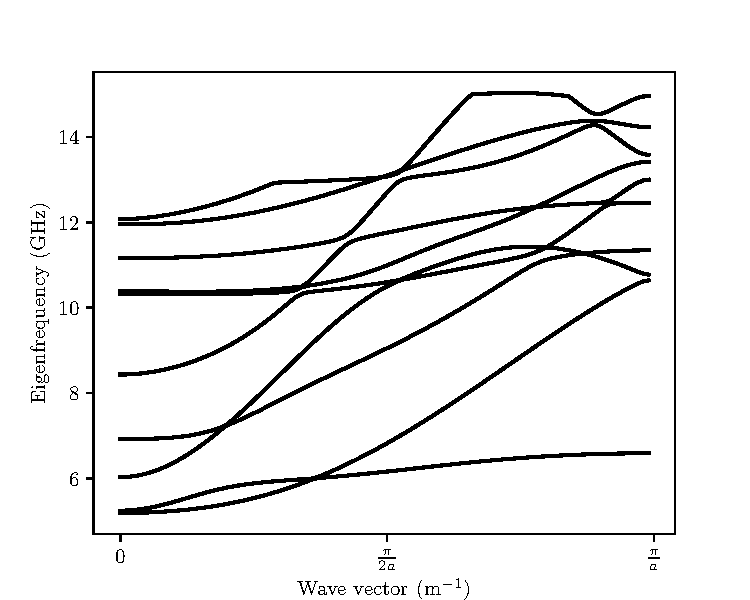
\includegraphics{chapters/theory/bandstructure.pdf}
	\caption{%
		Band diagram of phononic crystal defined in \cref{fig:unitcell}.
	}%
	\label{fig:banddiagram}
\end{figure}

\begin{figure}[htpb]
	\centering
	\begin{subfigure}[]{0.24\textwidth}
		\begin{center}
			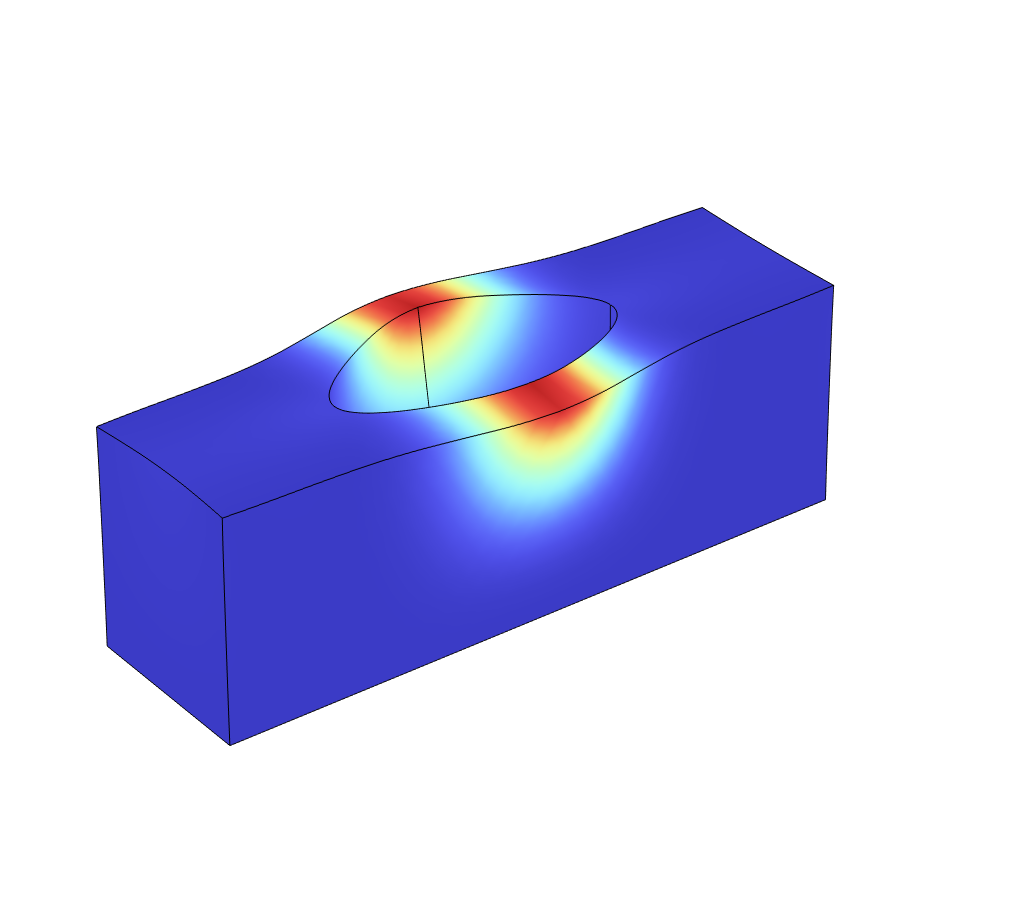
\includegraphics[width=\textwidth]{chapters/theory/modeshape_1.png}
		\end{center}
		\subcaption{}%
		\label{fig:ms1}
	\end{subfigure}
	\begin{subfigure}[]{0.24\textwidth}
		\begin{center}
			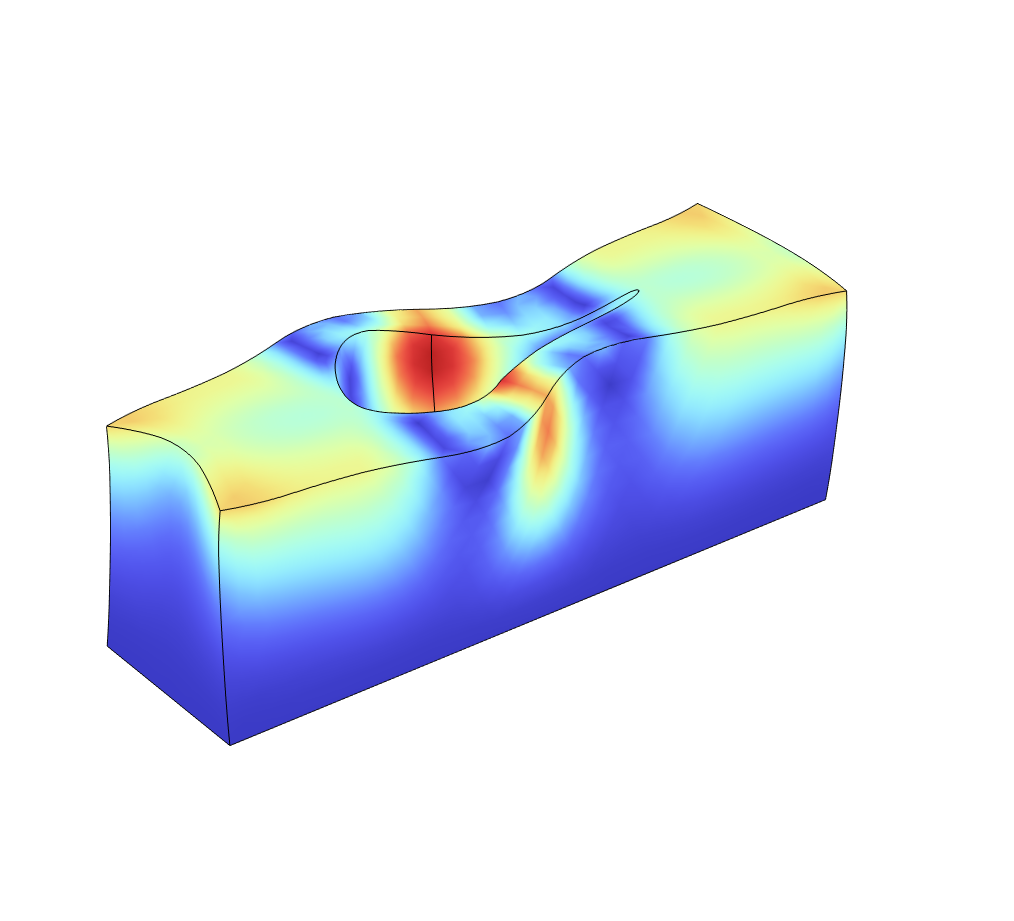
\includegraphics[width=\textwidth]{chapters/theory/modeshape_2.png}
		\end{center}
		\subcaption{}%
		\label{fig:ms2}
	\end{subfigure}
	\begin{subfigure}[]{0.24\textwidth}
		\begin{center}
			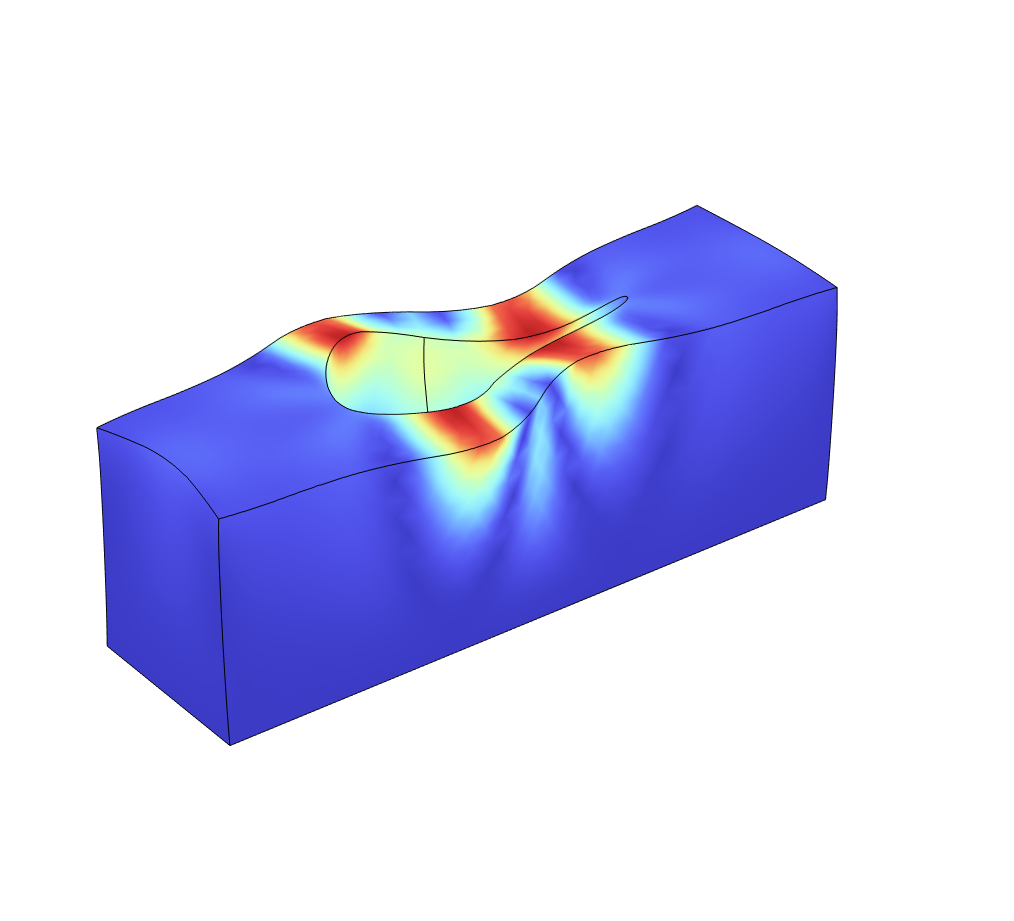
\includegraphics[width=\textwidth]{chapters/theory/modeshape_3.png}
		\end{center}
		\subcaption{}%
		\label{fig:ms3}
	\end{subfigure}
	\begin{subfigure}[]{0.24\textwidth}
		\begin{center}
			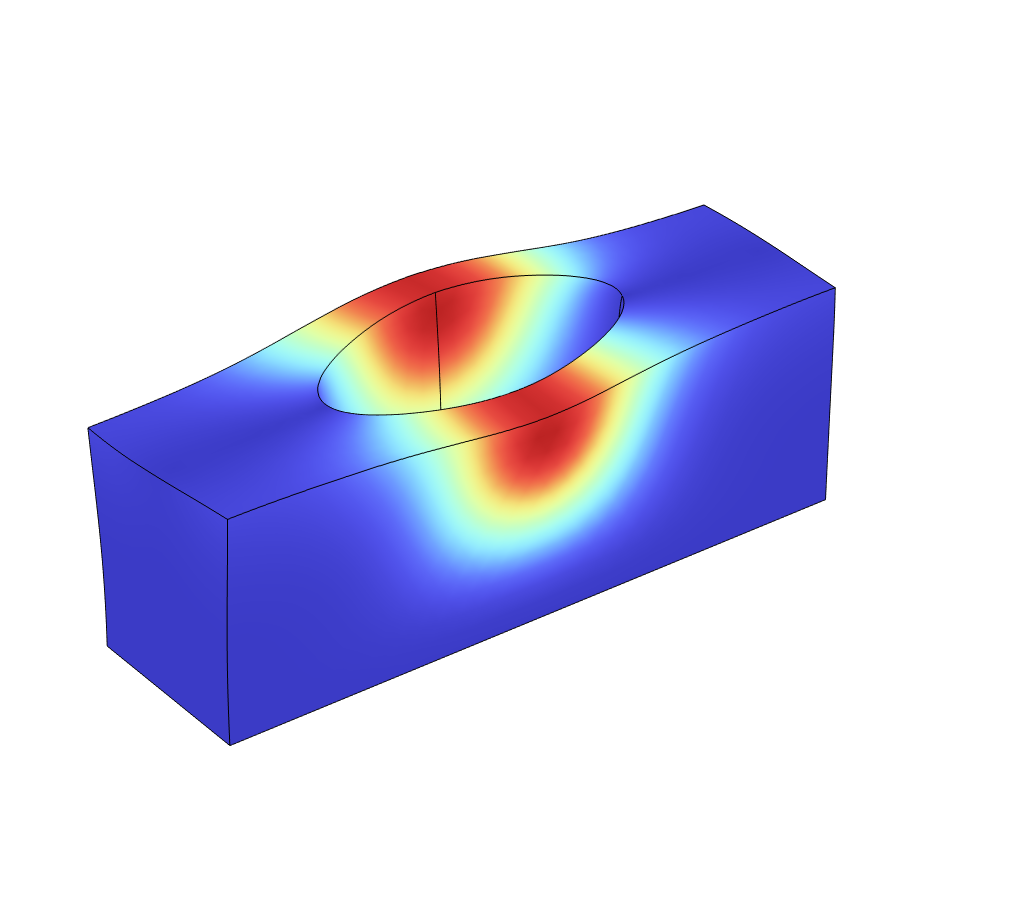
\includegraphics[width=\textwidth]{chapters/theory/modeshape_4.png}
		\end{center}
		\subcaption{}%
		\label{fig:ms4}
	\end{subfigure}\\

	\begin{subfigure}[]{0.24\textwidth}
		\begin{center}
			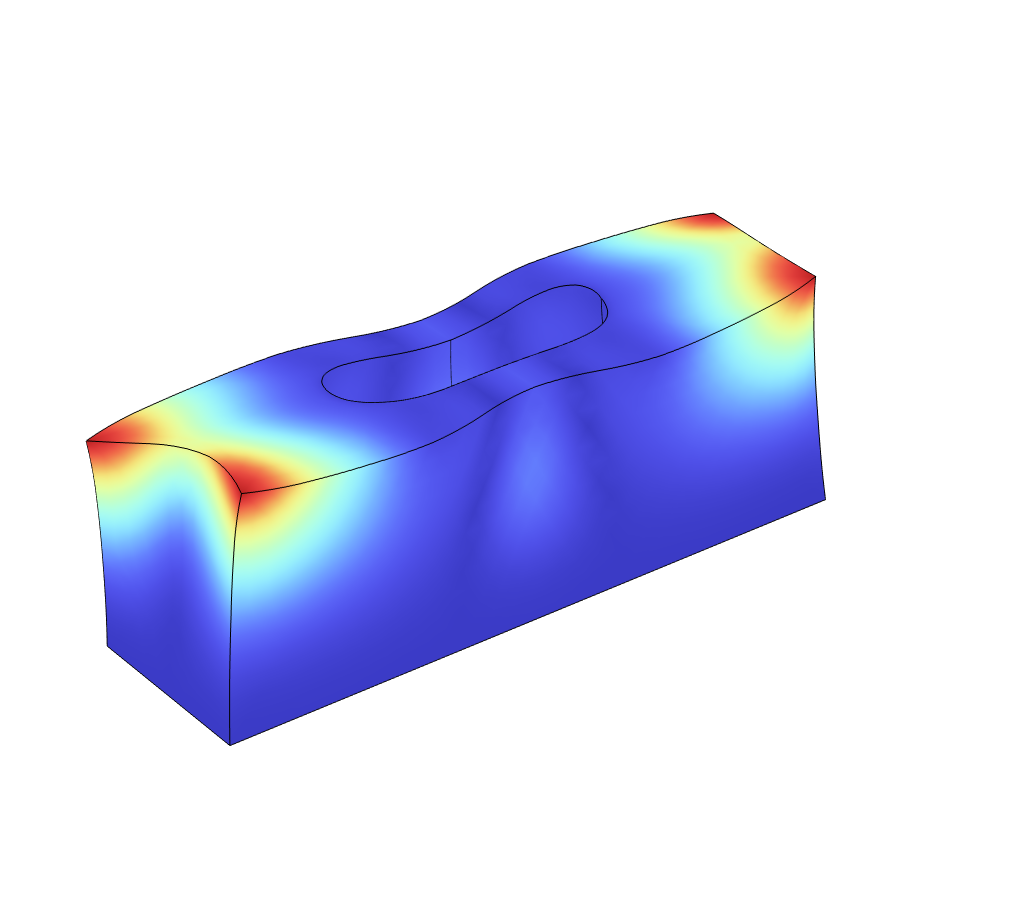
\includegraphics[width=\textwidth]{chapters/theory/modeshape_5.png}
		\end{center}
		\subcaption{}%
		\label{fig:ms5}
	\end{subfigure}
	\begin{subfigure}[]{0.24\textwidth}
		\begin{center}
			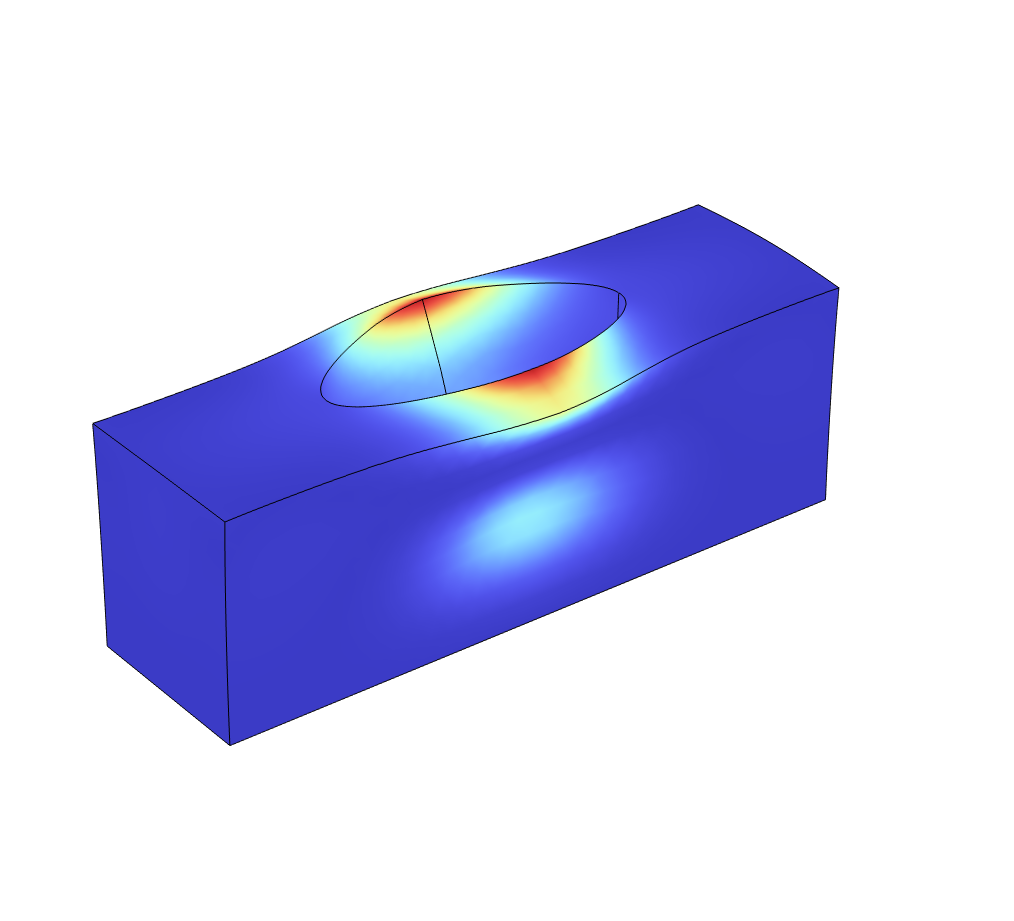
\includegraphics[width=\textwidth]{chapters/theory/modeshape_6.png}
		\end{center}
		\subcaption{}%
		\label{fig:ms6}
	\end{subfigure}
	\begin{subfigure}[]{0.24\textwidth}
		\begin{center}
			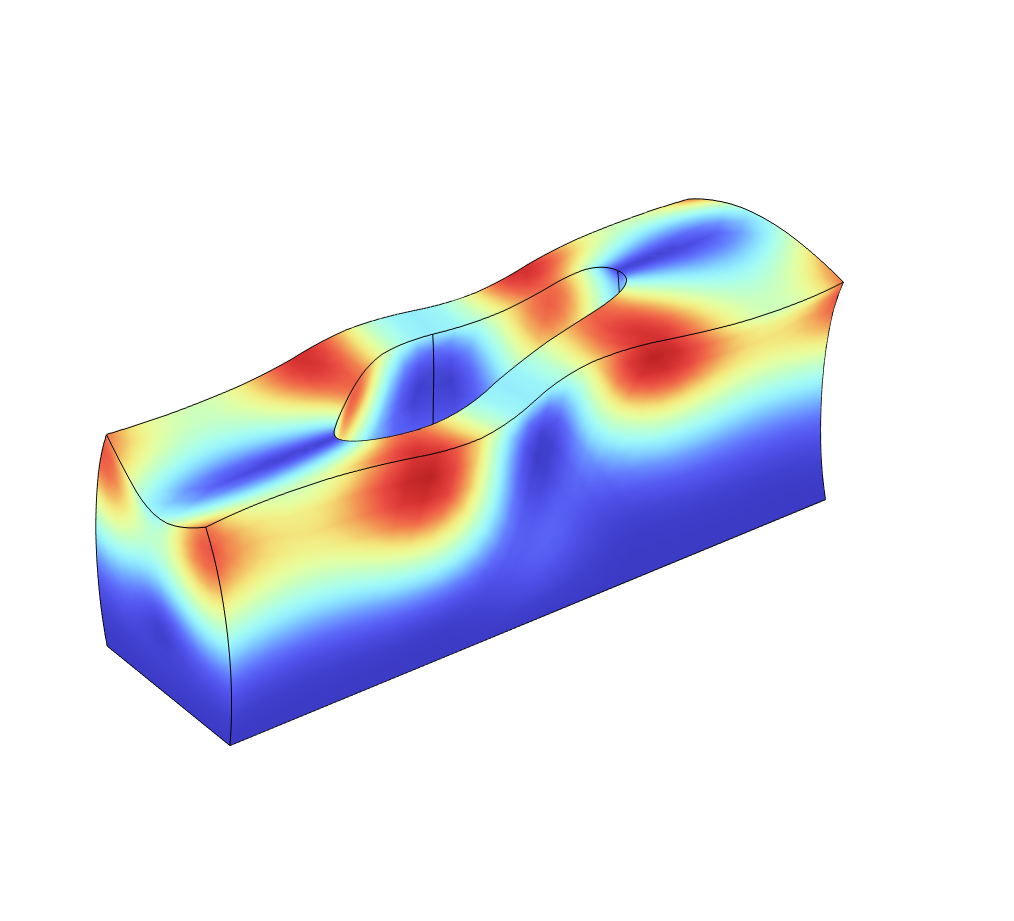
\includegraphics[width=\textwidth]{chapters/theory/modeshape_7.png}
		\end{center}
		\subcaption{}%
		\label{fig:ms7}
	\end{subfigure}
	\begin{subfigure}[]{0.24\textwidth}
		\begin{center}
			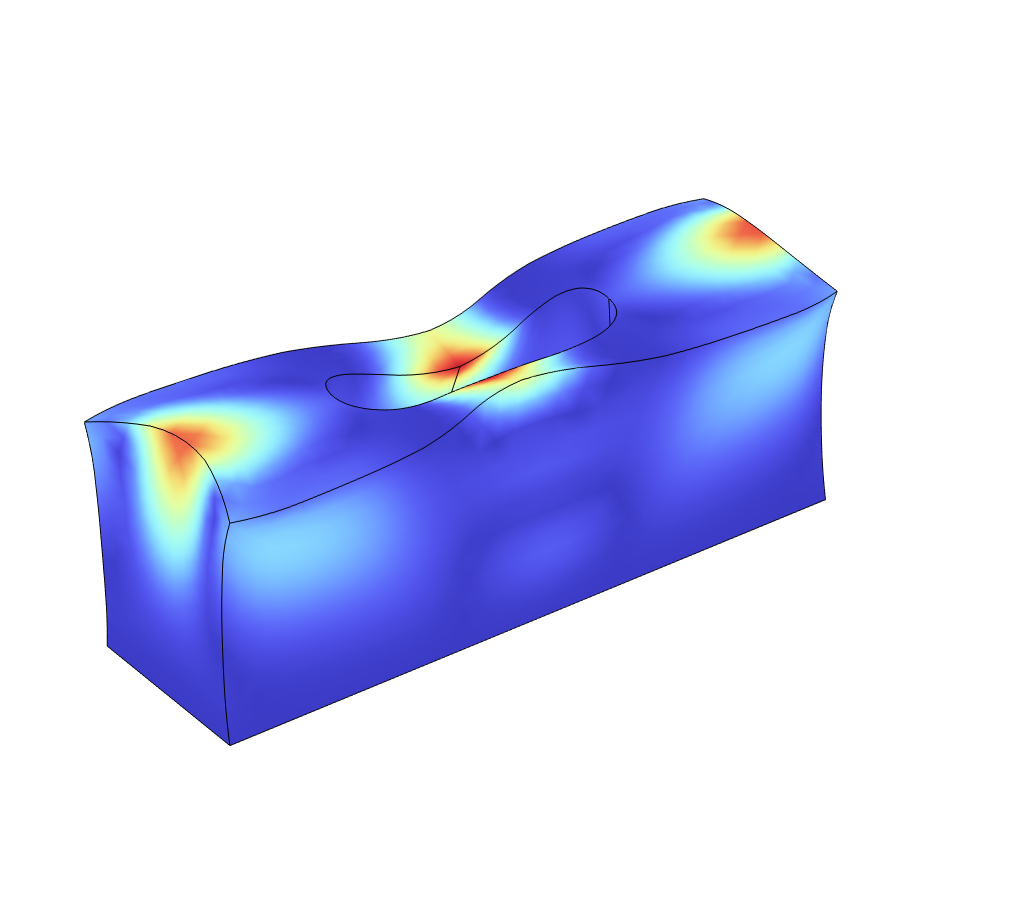
\includegraphics[width=\textwidth]{chapters/theory/modeshape_8.png}
		\end{center}
		\subcaption{}%
		\label{fig:ms8}
	\end{subfigure}

	\caption{%
		Mode shapes for the lowest eight modes at $k=0.9 \pi / a$.
		The color denotes the absolute value of the displacement,
		and the scale is normalized for each figure.
	}%
	\label{fig:modeshapes}
\end{figure}
\tododec{At some point write about phonons? I haven't really had to care about
the fact that excitations are discrete so if I talk about it it'd just for applications...}

\chapter{Inverse Design}

Inverse design is a design paradigm where the design of a device is guided fully by
the desired characteristics.
These desired characteristics are quantified through what is called an objective
function%
\footnote{Also called \emph{figure of merit (FoM)}.}%
, which I will denote $\fobj$,
that should be maximized.
When coupled with \emph{adjoint simulation}, which is a clever way to compute
gradients, and gradient based optimization
algorithms, this is a very powerful methodology.

An overview of the design process is as follows:
\begin{enumerate}
	\item Initialize a random device design.
	\item\label{it:grad} Calculate the gradient of the design through the adjoint method.
	\item Update the device design using the gradient according to the optimization algorithm.
	\item If the device performance is good enough, terminate optimization, else
		return to step~\ref{it:grad}.
\end{enumerate}

\section{Adjoint Simulation}

Adjoint simulation is a way to compute the gradient of $\fobj$ with respect to
the design, which in our case means with respect to the material parameters.
I will in this section first give a general derivation, following
reference~\cite{giles_introduction_2000}.
In \cref{sec:spec_der} I will then derive the specifics when applying this to
acoustics.

\subsection{General Derivation}\label{sec:general_derivation}

Let $\fobj$ be a function which depends on some high-dimensional vector $v$.
The vector $v$ can be calculated by solving the linear equation
$A v = b$, where $b$ is a fixed vector and $A$ is a matrix that depends on a
vector of design parameters $p$.
This could be the acoustics equation, but it might also be the analogous
equation for photonics, or something completely different like fluid dynamics.
I will refer to the process of solving this equation as a simulation, since for
this thesis it is solved through the simulation software COMSOL.
The overall goal is to find the parameters $p$ that maximize the objective
function $\fobj$.
The goal of adjoint simulation is to find $\diff{\fobj}{p}$.
This can be expanded through the chain rule as
\begin{equation}
	\diff{\fobj}{p} = \diff{\fobj}{v} \diff{v}{p}.
\end{equation}
To find the latter factor we do
\begin{align}
	\diff{}{p} [Av = b] &\implies \diff{A}{p} v + A \diff{v}{p} = 0\\
						&\implies A\diff{v}{p} = -\diff{A}{p}
						v.\label{eq:direct_dvdp_solve}
\end{align}
Thus, if we can find a $\tilde v$ such that
\begin{equation}\label{eq:vtilde}
	\diff{\fobj}{v} = \tilde v A
\end{equation}
then
\begin{align}
	\label{eq:dfdp_vtilde}
	\diff{\fobj}{p} &=
	\tilde v A \diff{v}{p}\\
	&=
	-\tilde v \diff{A}{p} v.
\end{align}
Finding $\tilde v$ from \cref{eq:vtilde} amounts to solving the so called
\emph{adjoint problem}:
\begin{equation}
	A^\dagger \tilde v^\dagger = \diff{\fobj}{v}^\dagger
\end{equation}
hence the name adjoint method.
As it turns out, $A$ is in many cases symmetric (or self-adjoint) which means that this is simply a normal
simulation but with $\difs{\fobj}{v}^\dagger$ as the source.
Thus, to obtain the derivative we just need to run an additional
simulation with a different input.

Now you might be wondering: what have we gained by this?
Let $n$ be the dimension of $v$, $m$ the dimension of $p$ and $l$ the dimension
of $b$.
This means that $A$ is a matrix with dimension $l\times n$ and $\difs{A}{p}$ is
a rank three tensor with dimension $m\times l\times n$.
Thus solving for $\difs{v}{p}$ from equation \cref{eq:direct_dvdp_solve}
means solving for an $n \times m$ matrix, which much more computationally
expensive than solving for just a vector of dimension $n$.

\subsection{Specific derivation with acoustics}\label{sec:spec_der}

Now we turn to the specific case of acoustic devices.
Here $A v = b$ is replaced by the acoustic field equation (\cref{eq:gov_eq}):
\begin{equation}\label{eq:sim_eq}
	\hat A_{ik} u_k = F_i.
\end{equation}
Instead of vectors, like we saw in \cref{sec:general_derivation}, these quantities are now functions%
\footnote{%
	Vector-valued funcitons, but that is not the important part here.
}
of $\vec x$.
Analogously to the vector of design parameters we now have a \emph{design field}
$p(\vec x)$,
and analogously to $\fobj$ being a function of a vector, this $\fobj$ is a
function of a function, i.e.\ a \emph{functional}.
For a quick overview of functionals and their derivatives, see
\cref{box:functionals}.

\begin{mybox}[breakable, parbox=false, label=box:functionals]{On functionals and their derivatives}
	\tododec{
		Big fat box on functionals and their derivatives. I think this should be
		included somewhere, since very few of my peers know what a functional
		derivative is... Not really sure how though. I kinda like the thought of
		putting it in a box like this.
		Alternatively, I could put it in an appendix.
	}
Our $\fobj$ is no longer a function, but rather a \emph{functional}, and thus
we need to use the functional derivative instead of the ordinary derivative.
One can think of a functional as a function of a function,
i.e.\ something that maps an element of a function space to a scalar number.
There are also functionals which depend on both a function and a real number,
or on multiple functions.
Below I will give an overview of the notational conventions I use,
and then give the definition of the functional derivative as well as some useful
properties of it.

Let $\mathcal{Y}$ be a function space of functions $\R \to \R$.
A functional $F:\mathcal{Y} \to \R$ evaluated at the function
$f\in\mathcal{Y}$
is denoted with the function in square brackets: $F[f]$.
Note that in principle, $F$ is the functional while $F[f]$ is just a
number,
analogously to how $f$ is a function while $f(x)$ is a real number.
If the functional additionally depends on a real number,
$G:\mathcal{Y} \times \R \to \R$,
that is put in round brackets: $G[f](x)$.

The functional derivative of $F$ with respect to its function argument
is a functional $\mathcal{Y} \times \R \to \R$ denoted $\difs.f.{F[f]}{f}$.
In this expression, $f$ is technically a dummy function, writing
$\difs.f.{F[g]}{g}$ is exactly the same functional.
However, often the argument of $F$ is omitted and the function in the
denominator is named in accordance with the names in the definition of the
functional.
Furthermore, the same notation is also often used to denote the functional
derivative evaluated at a certain function.
For example, if we define a functional taking two function arguments
$F[f_1, f_2] = \int f_1(x) + f_2(x) \dl x$, one can write
\begin{align}
	\diff.f.{F}{f_2}(x)
	&& \text{meaning}&\quad \diff.f.{F[g_1, g_2]}{g_2}(x)\\
	\diff.f.{F}{f_2}(x)
	&& \text{meaning}&\quad \diff.f.{F[g_1, g_2]}{g_2} [f_1, f_2](x)
\end{align}
where in the latter case, $f_1$ and $f_2$ are specific functions defined
previously.
Also note that the scalar argument to the functional derivative can be put
either in the denominator or after, depending on what is more convenient.
Oftentimes, when the functional being differentiated is a long expression and is
placed after the fraction, the argument is placed in the denominator:
\begin{equation}
	\diff.f.{F}{f}(x) = \diff.f.{F}{f(x)} = \diff.f.*{F}{f(x)}
\end{equation}

The functional derivative is defined by
\begin{equation}
	\int \diff.f.{F}{f} (x) \varphi(x) \dl x
	= \diff*{F[f + \varepsilon \varphi]}{\varepsilon}
\end{equation}
where $F$ is a functional of $f$ and $\varphi$ is an arbitrary test function.
I will use two properties of the functional derivative:
\begin{itemize}
	\item If $F$ is the functional $F[f](y) = f(y)$,
		then $\difs.f.{F(y)}{f}(x) = \delta(y-x)$.
	\item The chain rule: if $F$ is a functional with one function argument,
		$G$ is a functional with one function and one real argument,
		and $H$ is the functional defined as $H[f] = F[G[f](y)]$,
		then
		\begin{equation}
			\diff.f.{H}{f}(x)
			= \int \diff.f.{F}{G[f]}(y) \diff{G(y)}{f}(x) \dl{y}
		\end{equation}
\end{itemize}
\end{mybox}

For simplicity I will limit myself to the case where the objective function is
an overlap integral of the displacement field $u_k(\vec x)$ with some function
$\varphi_k^*(\vec x)$:
\begin{equation}
	\fobj[\vec u] = \int_\Omega u_i(\vec x) \varphi_i^*(\vec x) \dl{\vec x}.
\end{equation}
where $\Omega$ is the domain of $\vec u$.
Such an integral is an inner product in the space of functions on
$\Omega$.

Analogously to the general derivation in \cref{sec:general_derivation},
the chain rule is used to expand
$\difs.f.{\fobj}{p}(\vec x)$, see \cref{box:functionals} for the form of the
chain rule for the functional derivative.
However, because $\vec u$ is in general complex, I will split it into its real and
imaginary components: $\vec u = \vec v + i \vec w$.
\begin{equation}
	\label{eq:chain_rule}
	\diff.f.{f_\text{obj}}{p}(\bm x)
	=
	\int_\Omega \dl{\bm y} 
	\diff.f.{f_\text{obj}}{v_i}(\bm y)
	\diff.f.{v_i(\bm y)}{p}(\bm x)
	+
	\diff.f.{f_\text{obj}}{w_i}(\bm y)
	\diff.f.{w_i(\bm y)}{p}(\bm x)
\end{equation}
The first factor of each of the two terms is easy enough to calculate:
\begin{align}
	\diff.f.{f_\text{obj}}{v_i}(\bm y) &=
	\diff.f.*{
		\int_\Omega u_j(\bm x) \varphi_j^*(\bm x) \dl{\bm x}
	}{v_i(\bm y)}\\
	&= \int_\Omega
	\diff.f.*{
		u_j(\bm x) \varphi_j^*(\bm x)
	}{v_i(\bm y)} \dl{\bm x}\\
	&= \int_\Omega
	\delta(\bm x - \bm y) \delta_{ij} \varphi_j^*(\bm x)
	\dl{\bm x}\\
	&= \varphi_i^*(\bm y)
\end{align}
and
\begin{align}
	\diff.f.{f_\text{obj}}{w_i}(\bm y) &=
	\diff.f.*{
		\int_\Omega u_j(\bm x) \varphi_j^*(\bm x) \dl{\bm x}
	}{w_i(\bm y)}\\
	&= \int_\Omega
	\diff.f.*{
		u_j(\bm x) \varphi_j^*(\bm x)
	}{w_i(\bm y)} \dl{\bm x}\\
	&= \int_\Omega
	i \delta(\bm x - \bm y) \delta_{ij} \varphi_j^*(\bm x)
	\dl{\bm x}\\
	&= i \varphi_i^*(\bm y)
\end{align}
which gives us
\begin{align}
	\diff.f.{f_\text{obj}}{p}(\bm x)
	&=
	\int_\Omega \dl{\bm y}
	\varphi_i^*(\bm{y})
	\diff.f.{v_i(\bm y)}{p}(\bm x)
	+
	i \varphi_i^*(\bm{y})
	\diff.f.{w_i(\bm y)}{p}(\bm x)\\
	&=
	\int_\Omega \dl{\bm y}
	\varphi_i^*(\bm{y})
	\Re\left(\diff.f.{u_i(\bm y)}{p}(\bm x)\right)
	+
	i \varphi_i^*(\bm{y})
	\Im\left(\diff.f.{u_i(\bm y)}{p}(\bm x)\right)\\
	&=
	\int_\Omega \dl{\bm y}
	\varphi_i^*(\bm{y})
	\diff.f.{u_i(\bm y)}{p}(\bm x)
	\label{eq:dfdp_as_dudp_integral}
\end{align}
To find $\difs.f.{u_i(\bm y)}{p}(\bm x)$ we apply $\difs.f.{}{p(\bm x)}$ to
\cref{eq:sim_eq}, which gives us
\begin{equation}\label{eq:dAdpu_Adudp}
	0 =
	\diff.f.{\hat A_{ik}(\vec y)}{p}(\vec x) u_k(\bm y)
	+
	\hat A_{ik}(\vec y) \diff.f.{u_k(\bm y)}{p}(\bm x)
\end{equation}

% The point of inverse design is that we now want to find an adjoint field
% $\tilde u_i(\bm y)$
% such that the integral in \cref{eq:dfdp_as_dudp_integral} is
Just like \cref{eq:dfdp_vtilde},
we want an adjoint field $\tilde{\vec u}$
such that the integral in \cref{eq:dfdp_as_dudp_integral} is
\begin{equation}\label{eq:phi_dudp_integral}
	\int_\Omega \dl{\bm y}\,
	\varphi_i^*(\bm y)
	\diff.f.{u_i(\bm y)}{p}(\bm x)
	=
	\int_\Omega \dl{\bm y}\,
	\tilde u_i(\bm y)
	\hat A_{ik}(\vec y)
	\diff.f.{u_k(\bm y)}{p}(\bm x)
\end{equation}
which by \cref{eq:dAdpu_Adudp} is equal to
\begin{equation}\label{eq:an_integral}
	-\int_\Omega \dl{\bm y}\,
	\tilde u_i(\bm y)
	\diff.f.{\hat A_{ik}(\vec y)}{p}(\vec x)
	u_k(\bm y).
\end{equation}
The adjoint field is found by solving the adjoint problem:
\begin{equation}\label{eq:adjoint_problem}
	\hat A_{ik}^\dagger \tilde{u}_k = \varphi^*_i,
\end{equation}
where the adjoint operator $\hat A_{ik}^\dagger$ is defined through
\begin{equation}
	\int_\Omega f(\vec x) \left(\hat A_{ik}(\vec x) g(\vec x)\right) \dl{\vec x}
	=
	\int_\Omega \left(\hat A_{ik}^\dagger (\vec x)f(\vec x)\right) g(\vec x) \dl{\vec x}.
\end{equation}
To further simplify this expression, the dependence of $\hat A$ on $p$ must be
specified.
A linear dependence is proposed here, though extending the formula to more
complicated dependences is rather easy.
Taking $\rho(\vec y) = \rho^0 p(\vec y)$
and $C_{ijkl}(\vec y) = C_{ijkl}^0 p(\vec y)$
in the definition of $\hat A_{ik}$ from \cref{eq:A_def}
implies 
\begin{align}
	\diff.f.{\hat A_{ik}(\vec y)}{p}(\vec x)
	= -\rho^0 \omega^2 \delta_{ik} \delta(\vec x - \vec y)
	- \partial_j\left(C_{ijkl}^0\delta(\vec x - \vec y) \partial_l \placeholder\right)\\
	\label{eq:dadp}
	= -\rho^0 \omega^2 \delta_{ik} \delta(\vec x - \vec y)
	- 2 C_{ijkl}^0\delta(\vec x - \vec y)\partial_j \partial_l.
\end{align}
Plugging this back into the integral in \cref{eq:an_integral} gives
\begin{equation}
	\omega^2 \rho^0 \tilde u_i(\vec x) u_i(\vec x)
	+ 2 C_{ijkl}^0 \tilde u_i(\vec x) \partial_j \partial_l u_k(\vec x)
\end{equation}
which is comparatively easily evaluated.

Summarizing: in order to compute the gradient $\difs.f.{\fobj}{p}(\vec x)$ we first
run a normal simulation, i.e.\ solve \cref{eq:sim_eq}, to obtain $\vec u$.
Then we run an adjoint simulation, i.e.\ we solve \cref{eq:adjoint_problem}, to
obtain $\tilde{\vec u}$.
Finally, we calculate $\difs.f.{A(\vec y)}{p}(\vec x)$, which is given in
\cref{eq:dadp} in the case of a linear material parameter dependence on $p$,
and obtain the gradient through \cref{eq:an_integral}.
This gradient tells us \emph{at every point in the design} if $p$ should be
increased or decreased in order to increase $\fobj$.
The next section will describe more precisely how this is used to optimize the
design.

\section{Optimization Algorithms}

In this section I motivate why the gradient is so useful and how it will be
used in my algorithm.
I begin by describing the advantages of gradient based optimization
algorithms over those that don't use the gradient.
Following that I describe gradient descent, the most basic gradient based
optimization method, as well as \gls{adam}, which is the algorithm that I have
used.

An optimization algorithm is an algorithm for finding the optimum of a function.
The function is often called the \emph{objective function} or the \emph{cost
function}.
A very naive optimization method would be to simply try some number of inputs
and then choose the one with the highest function value.
This requires a large number of points before a good value is found,
meaning that it takes a long time.
An improvement to this method is to use the information gained from the points
already tried to decide which points to try next.
If some point has a bad value, then try somewhere else; if some point has a good
value, try another close by.
Examples of algorithms that do this are bayesian optimization, particle swarm
optimization, and various forms of genetic
algorithms~\cite{schneider2019benchmarking}.
However, if the domain of the objective function is very high-dimensional,
``close by'' is a very large space.
For such functions, it is essential to know in which direction the
function increases.
That is why gradient based optimization algorithms are so powerful;
they enable us to quickly find the right direction to go in for best
improvement.

% \tododec{%
% 	Curiosity that could be included:
% 	If you have a linear function (which all functions are if you zoom in far
% 	enough) $f(x) = v\cdot x + k$, and take a random step (random meaning random
% 	step in $[-\epsilon, \epsilon]$ in each dimension)
% 	then the expected improvement (given that you don't go downhill, in which
% 	case you can just stay where you are).
% 	% Curiosity that could be included. If you have a linear function
% 	% $f(x) = v\cdot x + k$, what is the probability that you will significantly
% 	% (say more than 10\% of optimal step) increase $f$ with a random unit
% 	% length step?
% 	% Optimal: step in $\hat v$, $\Delta f = v\cdot \hat v = \norm{v}$.
% 	% Probability of 10\% of this: $\int_{0.1}^1 (1-x^2)^{n/2} \dl x / \int_{-1}^1
% 	% \cdots$
% 	% use $(1-x^2)^n \approx \exp(-n x^2)$.
% 	% Approaches 0 very very quickly, at 10000 dimensions it's like \num{1e-45} or something.
% 	% Or maybe give the expected improvement given that you take the max of
% 	% current result and next result.
% }

\subsection{Gradient Descent}

The simplest gradient based optimization algorithm is called \emph{gradient
descent}.\footnote{%
	The reason for calling it gradient descent, instead of gradient ascent is
	simply a convention. Any maximization problem can be made into a
	minimization problem by multiplying that objective function by $-1$,
	so which formulation one chooses is arbitrary. However, the convention of
	talking about gradient descent is so strong that I will stick to that
	terminology, even though I am solving a maximization problem.%
}
Like all of the algorithms I will describe it is an iterative algorithm,
meaning that it generates a sequence of points that converges to an optimum,
and the next point in the sequence is derived from the previous ones.
In the case of gradient descent, the next point is gotten by
\begin{equation}
	p_n = p_{n-1} + \eta g_{n-1}
\end{equation}
where $\eta$ is the so called \emph{learning rate} and $g_{n-1}$ is the gradient
of the objective function at $p_{n-1}$.
For ordinary gradient descent the learning rate would be fixed,
and choosing an appropriate value for this parameter is one of the problems of
this method.
If a too high value is chosen, then the steps taken will be too large and the
optimium might be missed entirely.
A too low value results in too small steps which will yield a slow convergence.
Most gradient descent implementations nowadays use a so called learning schedule,
which means that $\eta$ is not constant during the optimization.
This introduces the additional problem of choosing how fast and between
which values it should change.

\subsection{Adaptive Moment Estimation (ADAM)}

The \gls{adam} algorithm is an improved version of gradient descent.
It has three main differences:
\begin{enumerate}
	\item Each dimension has a separate learning rate.
	\item The learning rate is automatically set from the previously seen gradients.
	\item The evolution carries some momentum.
\end{enumerate}
\Cref{fig:adam_vs_gd} shows the difference in performance between \gls{adam}
and \gls{gd}.
With a slightly too large learning rate, the \gls{gd} algorithm gets stuck in an
oscillation and makes very little progress towards the minimum.
If the learning rate is decreased, the oscillations disappear but the stepsize
is now too small to make it all the way to the true minimum. 
Since the \gls{adam} algorithm has some momentum, the motion along the valley
gets compounded while the motion perpendicular gets dampened which means that
the oscillations are not as much of a problem.
The adaptive learning rate also means that the algorithm doesn't get stuck
prematurely due to the small gradient at the bottom of the valley.
Admittedly, this objective function is specifically chosen to showcase the
advantages of \gls{adam}, but it has been shown to outperform \gls{gd} in almost
all cases~\cite{kingma2017adam}.
\begin{figure}[htpb]
	\centering
	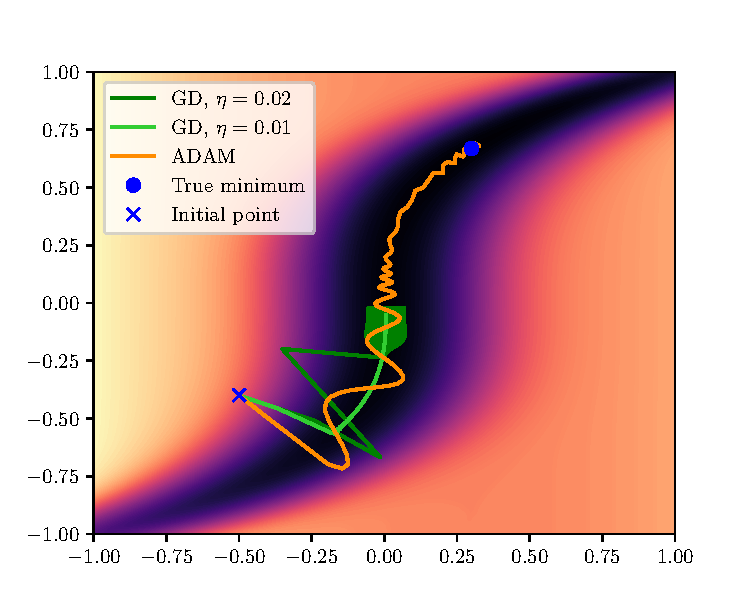
\includegraphics{chapters/theory/adam_vs_gd_plot.pdf}
	\caption{
		A comparison between \gls{adam} and \gls{gd} in an optimization
		landscape with a narrow canyon. The two different \gls{gd} algorithms
		are shown with 1000 steps, while 200 steps with the \gls{adam} algorithm
		are shown.
	}
	\label{fig:adam_vs_gd}
\end{figure}

\Cref{lst:adam} shows a pseudocode implementation of the \gls{adam} algorithm,
which has four important hyperparameters.
The first is $\alpha$ which controls the order of the step size.
The next $p$ will never be much further away than $\alpha$ in any dimension.
$\beta_1$ and $\beta_2$ control how quickly the momentum decays.
The algorithm basically keeps an exponentially decaying average of the previous
gradients and previous squared gradients.
The $\beta$:s set the decay rate for these averages.
Finally, there is $\epsilon$, which serves to make the algorithm more stable.
If the average magnitude of the gradient becomes much smaller than $\epsilon$,
the algorithm will slow down.

\begin{listing}
	\begin{minted}{Python}
def adam(p_0, get_gradient, alpha,
		beta_1, beta_2, epsilon, n_iter):

	m = np.zeros(theta_0.shape)
	v = np.zeros(theta_0.shape)
	p = p_0

	for i in range(n_iter):
		g = get_gradient(theta)
		# Update biased first moment estimate
		m = beta_1 * m + (1-beta_1) * g
		# Update biased second moment estimate
		v = beta_2 * v + (1-beta_2) * g**2

		# Compute the bias-corrected estimates
		m_hat = m / (1 + beta_1**i)
		v_hat = v / (1 + beta_2**i)

		# Update p
		p += alpha * m_hat / (np.sqrt(v_hat) + epsilon)
	\end{minted}
	\caption{%
		Pseudocode for the ADAM algorithm. See \cite{kingma2017adam} for a more
		in depth discussion of the algorithm.
	}
	\label{lst:adam}
\end{listing}

\chapter{Methods}\label{sec:methods}

The aim of this thesis is to use inverse design to find a phononic beamsplitter,
a task that can be divided into three parts: 
First, some definitions of what
should be designed and what constitutes a ``good'' design needs to be made.
Second, we need a way to calculate the gradient of the ``goodness'' with respect
to the design.
And lastly, we need a gradient based optimization algorithm to find the optimal
design.
All of this will be described in this chapter.

\section{Design}

The device design to be optimized can be seen in \cref{fig:bs-design}.
The input and output waveguides consists of unit cells like the one in
\cref{fig:unitcell}.
The values for the parameters in the sketch are given in \cref{tab:params}.
The reason for using this mode in this waveguide is that it has been shown to be
interesting for avoiding mechanical leakage into the substrate on which it is
clamped, as well as retaining a high optomechanical
coupling.\cite{kolvik_clamped_2023}

Inside the design area, there can be one of two kinds of designs.
The first is a \emph{continuous design}, meaning that the material parameters
$\rho$ and $C_{ijkl}$ are continuously varying. The range of values that they
can take are between the density and elasticity of pure silicon and that of air.
Any in-between values are obviously not something that can be physically
realized, but it is useful as a first step in the optimization.
This is parametrized through the \emph{design field}, $p$, which takes values
between 0, which means pure air, and 1, which means pure silicon.
The second kind is a binary design, where each point either has silicon or not
and there are no in-between values.
This is accomplished using level-set methods, which will be explained in
\cref{sec:level-set}.

Because the device is completely symmetric, only one half of it needs to be
modeled, and the other half is extrapolated with a symmetry boundary condition.

\begin{figure}[htpb]
	\centering
	\def \a{0.5}
\def \w{1.0}
\def \hx{0.13}
\def \hy{0.3}

\tikzset{
	unitcell/.pic={
		\draw[pic actions] (-0.5*\a, -0.5*\w) rectangle (0.5*\a, 0.5*\w);
		\draw[fill=white] (0, 0) circle [x radius=\hx, y radius=\hy];
	}
}

\begin{tikzpicture}[scale=0.7]
	\def \designx{4.0}
	\def \designy{4.0}
	\def \outputh{1.0}
	\def \nunitcells{16}
	\def \nnonpmls{10}

	% Coordinate system
	\draw[gray, thick, ->] (0,0) -- (0,-1) node [anchor=west] {$x$};
	\draw[gray, thick, ->] (0,0) -- (1,0) node [anchor=west] {$y$};

	% Input waveguide
	\path
		(-0.5*\a, 0) pic[transform shape] {unitcell}
		(-1.5*\a, 0) pic[transform shape] {unitcell}
		(-2.5*\a, 0) pic[transform shape] {unitcell}
		(-4.0*\a, 0) node {$\cdots$}
		(-5.5*\a, 0) pic[transform shape] {unitcell}
		(-6.5*\a, 0) pic[transform shape] {unitcell}
		(-7.5*\a, 0) pic[transform shape] {unitcell};
	\draw[red, ultra thick]
		(-7*\a, -0.5*\w) --
		(-7*\a, +0.5*\w);
	\begin{scope}[dash=on 1pt off 1pt phase 0pt]
	\path
		(-8.5*\a, 0) pic[transform shape] {unitcell}
		(-9.5*\a, 0) pic[transform shape] {unitcell}
		(-10.5*\a, 0) pic[transform shape] {unitcell}
		(-12.0*\a, 0) node {$\cdots$}
		(-13.5*\a, 0) pic[transform shape] {unitcell};
	\end{scope}

	% Design area
	\draw (0, -\designx / 2) rectangle (\designy, \designx / 2);
	\node at (\designy / 2, 1) {Design Area};
	\node[left] at (\designy, 0) {$d_x$};
	\node[above] at (\designy/2, -\designx/2) {$d_y$};

	% Output waveguide
	\begin{scope}[xshift=\designy cm, yshift=\outputh cm]
	\path
		(0.5*\a, 0) pic[transform shape] {unitcell}
		(1.5*\a, 0) pic[transform shape] {unitcell}
		(2.5*\a, 0) pic[transform shape] {unitcell}
		(4.0*\a, 0) node {$\cdots$}
		(5.5*\a, 0) pic[transform shape] {unitcell}
		(6.5*\a, 0) pic[transform shape] {unitcell}
		(7.5*\a, 0) pic[transform shape, fill=blue] {unitcell};
	\begin{scope}[dash=on 1pt off 1pt phase 0pt]
	\path
		(8.5*\a, 0) pic[transform shape] {unitcell}
		(9.5*\a, 0) pic[transform shape] {unitcell}
		(10.5*\a, 0) pic[transform shape] {unitcell}
		(12.0*\a, 0) node {$\cdots$}
		(13.5*\a, 0) pic[transform shape] {unitcell};
	\end{scope}
	\end{scope}
	\begin{scope}[xshift=\designy cm, yshift=-\outputh cm]
	\path
		(0.5*\a, 0) pic[transform shape] {unitcell}
		(1.5*\a, 0) pic[transform shape] {unitcell}
		(2.5*\a, 0) pic[transform shape] {unitcell}
		(4.0*\a, 0) node {$\cdots$}
		(5.5*\a, 0) pic[transform shape] {unitcell}
		(6.5*\a, 0) pic[transform shape] {unitcell}
		(7.5*\a, 0) pic[transform shape, fill=blue] {unitcell};
	\begin{scope}[dash=on 1pt off 1pt phase 0pt]
	\path
		(8.5*\a, 0) pic[transform shape] {unitcell}
		(9.5*\a, 0) pic[transform shape] {unitcell}
		(10.5*\a, 0) pic[transform shape] {unitcell}
		(12.0*\a, 0) node {$\cdots$}
		(13.5*\a, 0) pic[transform shape] {unitcell};
	\end{scope}
	\end{scope}
	\draw[|-|]
		(15*\a + \designy, -\outputh) -- node[right] {$s$}
		(15*\a + \designy, \outputh);
		
\end{tikzpicture}

	\caption{
		Device design to be optimized.
		At the red line, a wave traveling right is excited.
		The output is measured over the blue unit cells.
		The dashed unit cells are \glspl{pml}.
		The large, rectangular design area has dimensions $d_x \times d_y \times
		h$.
	}
	\label{fig:bs-design}
\end{figure}

\begin{table}[htpb]
	\centering
	\caption{%
		Values for the geometric parameters of the device.
		Reference \cref{fig:bs-design,fig:unitcell} for what the quantities
		mean.
	}%
	\label{tab:params}

	\begin{tabular}{cc}
		\toprule
		Parameter & value\\
		\midrule
		$a$ & \qty{187}{\nm}\\
		$w$ & \qty{187}{\nm}\\
		$h_x$ & \qty{153.5}{\nm}\\
		$h_y$ & \qty{49.5}{\nm}\\
		$h$ & \qty{220}{\nm}\\
		$d_x$ & $6 w$\\
		$d_y$ & $4 w$\\
		$s$ & $3 w$\\
		\bottomrule
	\end{tabular}
\end{table}

\subsection{Objective function}

The figure of merit of the device is how much of the input excitation gets transmitted
into the output beams.
Furthermore, all of the excitation of the output waveguide should be in the same
mode that was excited at the input.
Therefore, a mode overlap integral is used:
\begin{equation}
	I = \int_{\Omega_1} \vec{u}(\vec{x}) \cdot \vec{u}_m^*(\vec{x}) \dl{\vec x},
\end{equation}
where $\vec u_m$ is the shape of the mode (\cref{fig:ms1}).
Because we are not interested in the phase of the output waves,
the absolute value squared of the overlap integral is taken as the objective
function,
\begin{equation}
	\fobj = \abs{I}^2 = I I^*.
\end{equation}
This will be maximal when the excitation of the mode $m$ in the output
waveguide is maximized, regardless of which phase it has.

The functional derivative of $\fobj$ with respect to $p$ then becomes
\begin{align}
	\diff.f.{\fobj}{p}(x) &= \diff.f.{I}{p}(x) I^* + I\diff.f.{I^*}{p}(x)\\
	&= \diff.f.{I}{p}(x) I^* + \left(I^*\diff.f.{I}{p}(x)\right)^*\\
	&= 2\Re\left(\diff.f.{I}{p}(x) I^*\right).
\end{align}
The derivative of $I$ was derived in \cref{sec:spec_der}.

\subsection{Excitation}\label{sec:excitation_method}

In order to excite the input waveguide in the desired mode,
the stress on the boundary of a unit cell was exported from a unit cell
eigenmode simulation with $k=0.9 \pi / a$ and applied to the boundary marked in red in
\cref{fig:bs-design}.
Since the frequency is perfectly controlled, this should excite only the desired
mode, since that is the only permitted mode close by as seen in the band diagram
in \cref{fig:banddiagram}.

In order to confirm that the excitation was indeed fully in the desired mode, a
separate model with only a waveguide with 200 unitcells was created.
After applying the excitation and running the simulation,
the proportion of the excitation that ended up in the desired mode was
calculated.
This was done by first calculating the mode overlap integral
$\int \vec u \vec u_m^* \dl{\vec x}$
and comparing that to the norm of the displacement field
$\int \vec u \vec u^* \dl{\vec x}$.
If we write $\vec u$ as $\vec u = a \vec u_m + b \vec u_r$ for some scalars $a$ and $b$,
then
$\int \vec u \vec u^* \dl{\vec x} = a\int \vec u \vec u_m^*\dl{\vec x} + b\int
\vec u \vec u_r^*\dl{\vec x}$.
And assuming $\vec u_r$ is orthogonal to $\vec u_m$,
$a = \int \vec u \vec u_m^*\dl{\vec x} / \int \vec u_m \vec u_m^*\dl{\vec x}$,
which enables us to calculate $b$ as well.
The result was near perfect ($b < 0.03 a$) excitation of only the desired mode.
Since energy is proportional to
the square of the amplitude, $b < 0.03 a$ means that $>99.9 \%$ of the energy was
in the correct mode.
To obtain such high fidelity, it was important that the mesh used for the
unitcells in the wave guide was the same as the mesh in the unit cell
simulation.
High fidelity was also achieved if both meshes were made very fine, but such
fine meshes carries a prohibitively large computational cost.

\subsection{Perfectly Matched Layers (PMLs)}

Ideally, the input and outputs are infinite waveguides.
Unfortunately, simulating infinite waveguides would take infinite time.
Instead, \glspl{pml} are placed at the caps of the input and output waveguides.
The purpose of the \gls{pml} is to absorb any incoming waves without reflection,
which would make it act as if there was an infinite waveguide on the other side
into which the waves propagate indefinitely.
The way to accomplish this is to add an imaginary component to the density of
the material.
\todowrt{why does it work}
The imaginary part must be introduced smoothly,
otherwise the abrupt change in material
parameters would induce reflections anyway.
Therefore, the imaginary part is taken to be exponentially increasing,
starting at $y_0$ and continuing until the end of the waveguide, $n$ unit cells
later.
Furthermore, the curve is shifted vertically such that it is 0 at $y = y_0-n$,
and rescaled so that it is $\rho_\text{si} s$ at $y=y_0$.
\begin{equation}
	\rho_\text{im} = \rho_\text{si} \cdot s \cdot
	\frac{e^{-\abs{y-y_0} / d} - e^{-n/d}}{1 - e^{-n/d}}
\end{equation}
\Cref{fig:pml_profile} shows the effect of changing these parameters on the
shape of the profile of the imaginary component.

\begin{figure}[htpb]
	\centering
	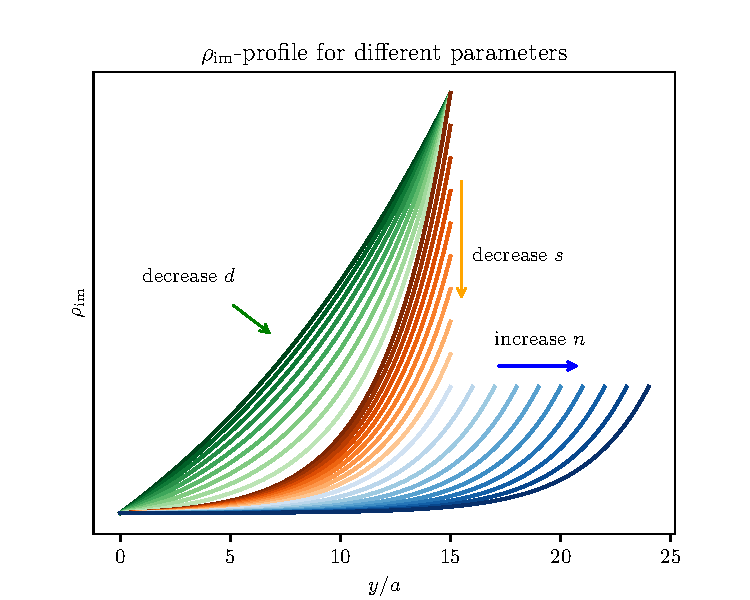
\includegraphics{chapters/methods/pml_profile.pdf}
	\caption{%
		This figure shows the effect of changing different parameters.
		The green curves shows changing $d$ while keeping the other parameters
		fixed, and the orange and blue show $s$ and $n$ respectively.
		Darker colour means higher value, and the last green curve coincides
		with the first orange, and the last orange with the first blue.
	}%
	\label{fig:pml_profile}
\end{figure}

There are three possible sources of reflections.
Firstly, if the transition from no imaginary component to some imaginary
component is too abrupt, that causes reflections.
Secondly, if the imaginary component is too small, the waves will not be
dampened completely when they reach the end of the \gls{pml} and thus reflect
off of that.
And lastly, if $d$ is small then there can be reflections from the steep
increase that happens some distance away from the beginning of the \gls{pml}.
See \cref{fig:banddiagram} for an illustration of where the different types of
reflections occur.

\tikzset{
	reflection/.pic={
		\draw[->] (-0.4, 0) -- (-0.1, 0) arc[radius=0.1, start angle=-90, end
		angle=90] --++ (-0.1, 0);
		\draw[dashed] (0,-3.1) -- (0,8.3);
	}
}
\begin{figure}[htpb]
	\centering
	\begin{tikzpicture}[domain=1:8]

		\draw[->,very thick] (-0.0,0) -- (8.2,0) node[right] {$y$};
		\draw[->,very thick] (0,-0.0) -- (0,4.2) node[above] {$\rho_\text{im}$};
		\draw[very thick] (1,0) -- (1,-0.10) node[below] {$y_0-n$};
		\draw[very thick] (7.9,0) -- (7.9,-0.10) node[below] {$y_0$};
		%\draw[very thin,color=gray] (-0.1,-1.1) grid (7.9,3.9);
		\clip (0.0, 0.0) rectangle (7.9,3.9);
		\draw[color=ForestGreen, very thick] (0,0) -- (1,0) --
			plot (\x,{0.40*(exp(\x/3)-exp(1/3))});
		\draw[color=Orange, very thick] (0,0) -- (1,0) --
			plot (\x,{0.10*(exp(\x/4)-exp(1/4))});
		\draw[color=NavyBlue, very thick] (0,0) -- (1,0) --
			plot (\x,{0.02*exp(2.0*(\x-4))});
		\draw[ForestGreen] (1.0, 0.3) pic {reflection};
		\draw[NavyBlue] (5.7, 0.8) pic {reflection};
		\draw[Orange] (7.9, 0.9) pic {reflection};
	\end{tikzpicture}
	\caption{%
		For the green curve, the initial sudden increase of the imaginary
		component of the density at the beginning of the \gls{pml} causes reflections.
		For the blue curve, the beginning of the \gls{pml} is smooth but there
		is an increase partway through sharp enough to cause reflections.
		For the orange curve, the \gls{pml} never becomes strong enough to
		completely dampen the waves, and they get reflected at the end.
	}%
	\label{fig:pml_reflections}
\end{figure}

It is desirable to make $n$ as small as possible while still eliminating all
reflections. In order to do so, a long waveguide with the same parameters as
used for the input and output waveguides in the beamsplitter design was created.
To discern where there was some component of the wave reflected, a fourier
transform of the displacement field was made.
The parameters controlling the shape of the $\rho_\text{im}$ curve were then
varied and an appropriate value was selected.

\subsection{Level-set}\label{sec:level-set}

Ultimately, we want our device to consist of regions of material and regions of
no material.
There are basically two ways of doing this.
The first, and perhaps most intuitive,
is to simply store the coordinates of the boundary between the filled and empty
regions.
In addition to storing the coordinates, one must also store which points
neighbour which.
The second method, which is the one used in this report, is called
the \emph{level-set method}.
In this method, the boundary is not directly stored, but rather is stored via an
\emph{implicit function}, $\phi(x)$, defined such that the boundary is the
0-isocontour of $\phi$, i.e.\ the points $x$ where $\phi(x)=0$.

There are two main advantages of using the level-set method rather than
directly storing the boundary points.
Firstly, when moving the boundary we would like to do so in the normal
direction, as moving it along itself has no effect.
Computing the normal direction of a directly stored boundary is slightly cumbersome,
though certainly achievable.
With level-set, moving the boundary in the normal direction is as easy as adding
a constant to the implicit function.
Secondly, while the boundary is changing, the resolution in one part might need
to be increased while the resolution in another needs to be decreased. Deciding
where and when to add new points is non-trivial when directly storing the
boundary. Furthermore, if two boundaries merge, or if one splits in two, points
need to be removed and the connectivities changed, which is quite complex.
\Cref{fig:direct_troubles} illustrates these problems with direct storage concretely.
Both of these issues are automatically handled with the level-set method.
\tododec{How? (Isn't it obvious?)}

\begin{figure}[htpb]
	\centering
	\begin{tikzpicture}[scale=1.5, very thick]
	\coordinate (ca) at (0,0);
	\coordinate (cb) at (1,0);
	\def\radiusa{0.7cm}
	\def\radiusb{0.1cm}
	\def\radpt{0.7pt}
	\draw (-1,-1) rectangle (1.5,1);
	\foreach \i in {0,15,...,360}{% 
		\filldraw [blue]  (ca)++(\i:\radiusa) circle (\radpt);
	}
	\foreach \i in {0,72,...,360}{% 
		\filldraw [blue]  (cb)++(\i:\radiusb) circle (\radpt);
	}
	\draw (ca) circle[radius=\radiusa];
	\draw (cb) circle[radius=\radiusb];

	\begin{scope}[xshift=3cm]
		\coordinate (ca) at (0,0);
		\coordinate (cb) at (1,0);
		\def\radiusa{0.4cm}
		\def\radiusb{0.4cm}
		\draw (-0.8,-1) rectangle (1.7,1);
		\foreach \i in {0,15,...,360}{% 
			\filldraw [blue]  (ca)++(\i:\radiusa) circle (\radpt);
		}
		\foreach \i in {0,72,...,360}{% 
			\filldraw [blue]  (cb)++(\i:\radiusb) circle (\radpt);
		}
		\draw (ca) circle[radius=\radiusa];
		\draw (cb) circle[radius=\radiusb];
	\end{scope}
	\begin{scope}[xshift=6cm]
		\coordinate (ca) at (0.2,0);
		\coordinate (cb) at (0.8,0);
		\def\radiusa{0.4cm}
		\def\radiusb{0.4cm}
		\draw (-0.8,-1) rectangle (1.7,1);
		\foreach \i in {60,75,...,315}{% 
			\filldraw [blue]  (ca)++(\i:\radiusa) circle (\radpt);
		}
		\foreach \i in {-72,0,72}{% 
			\filldraw [blue]  (cb)++(\i:\radiusb) circle (\radpt);
		}
		\foreach \i in {-45, -30, ..., 45}{% 
			\filldraw [red]  (ca)++(\i:\radiusa) circle (\radpt);
		}
		\foreach \i in {144, -144}{% 
			\filldraw [red]  (cb)++(\i:\radiusb) circle (\radpt);
		}
		\draw (ca)++(60:\radiusa)
			arc[radius=\radiusa, start angle=60, end angle=300]
			to[out=30, in=150]
			([shift=(240:\radiusb)] cb)
			arc[radius=\radiusb, start angle=240, end angle=480]
			to[out=210, in=-30]
			cycle;
		%\draw (cb) circle[radius=\radiusb];
	\end{scope}
\end{tikzpicture}

	\caption{%
		Possible evolution of boundary. In the leftmost figure, the
		boundary is defined by pretty much evenly spaced points. In the center figure
		the boundaries have moved and the spacing is no longer even, and the
		right circle is very poorly resolved.
		The rightmost figure shows the boundary after the two circles moved
		closer together. Now there are multiple points that need to be removed,
		marked in red, and the connectivity of the points that remain must be
		changed such that the two boundaries are merged.
	}%
	\label{fig:direct_troubles}
\end{figure}
\begin{figure}[htpb]
	\centering
	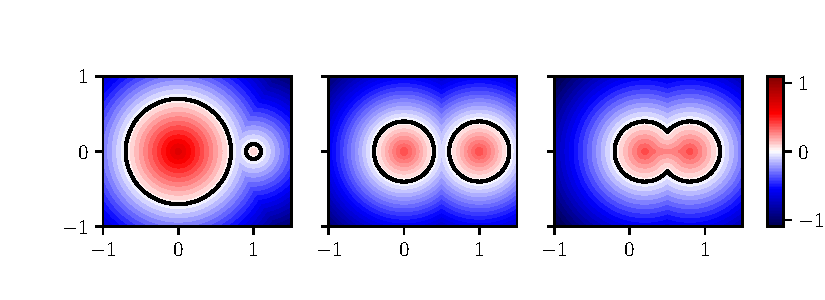
\includegraphics{chapters/methods/signed_dist_example.pdf}
	\caption{%
		Example of three signed distance functions for three different
		boundaries.
	}%
	\label{fig:signed_dist_example}
\end{figure}

There are of course a lot of possible functions $\phi(x)$ that have a given
boundary as it's 0-isocontour.
There is one choice that simplifies a lot of calculations though: the signed
distance function.
This function is defined as the distance from the closest point on the boundary,
with a plus sign if it is inside and a minus sign if it is outside the boundary.
See \cref{fig:signed_dist_example} for an example.
It has the advantage that if one wishes to locally shift the boundary some
length $s$ in the normal direction, then simply add $s$ to the function there.
\Cref{fig:add_shift} shows this effect in one dimension.
\todowrt{%
	Create another figure that shows it in two dimensions.
	I'm thinking a circular boundary, and adding $s$ in the left half and
	subtracting $s$ in the right half. Alternatively adding $s\cdot x$ (unit circle
	centered on 0) so that it will be smooth
}

\begin{figure}[htpb]
	\centering
	\begin{tikzpicture}[domain=0:3]
		\draw[very thin,color=gray] (-0.1,-2.1) grid (2.9,1.9);

		\draw[->] (-0.2,0) -- (3.2,0) node[right] {$x$};
		\draw[->] (0,-2.2) -- (0,2.2) node[above] {$\phi$};
		\draw[color=blue!50, dashed, very thick] plot (\x,{\x-2})
			node[right] {$\phi(x)$};
		\draw[color=blue, very thick] plot (\x,{\x-1})
			node[right] {$\phi(x)+s$};
		\filldraw[color=blue!50] (2,0) circle[radius=2pt];
		\filldraw[color=blue]    (1,0) circle[radius=2pt];
		\draw[color=red, ->, very thick] (1.9,0) --
			node[below] {$s$}
			(1.1,0);
	\end{tikzpicture}
	\caption{Adding $s$ to the signed distance function shifts boundary by
	$s$.}%
	\label{fig:add_shift}
\end{figure}

Using a signed distance function means that a gradient descent step can be taken
by simply adding the gradient field to the signed distance field.
However, there are some pitfalls that must be avoided.
Firstly, the gradient needs to be rescaled so that the boundary moves
an appropriate distance.
This has been done such that the boundary moves maximally \qty{1}{\nm}.
\todoblk[noinline]{check this number before finalizing, I change it every now and then}
Secondly, since the gradient is occasionally sharply peaked somewhere which may
not lie near the boundary, only the gradient near the boundary is actually added
to the signed distance field.
After performing this addition, what was previously a signed distance field will
now no longer be that, and thus the signed distance field is recalculated from
the new boundary.
This recalculation comes with a performance penalty, but since the COMSOL
simulations are orders of magnitude slower than all other parts of the
optimization, this is of little concern.


\section{Optimization}\label{sec:m_optimization}

For the optimization in the case of continuous optimization, the \gls{adam}
algorithm with one modification: a global learning rate was employed rather than
individual learning rates. The reasoning for this was that individual learning
rates would give jagged contours, which wouldn't be properly resolved by the
meshing. Practically this modification means that \mintinline{Python}+v+ is a
scalar and is set to \mintinline{Python}{(1-beta_2)*np.mean(g**2) + beta_2 * v}
in \cref{lst:adam}.
The optimization was run and continually monitored, and once convergence was
visually confirmed through looking at the plot of $\fobj$ by iteration, it was terminated.
A few different values for the $\beta$:s were tried, and in the end
$\beta_1=0.9$ and $\beta_2 = 0.95$ were chose. However, it seemed that the
evolution were not too sensitive to this choice.
$\alpha$ was taken to be \num{2e-3}, because that is large enough that $p$
could change from 0 to 1 in 500 iterations, which was deemed an appropriate
timescale since that took about one day.

The final step of the optimization was to use level-set for the design.
However, just using the final device of the continuous optimization for the
initial point of the level-set optimization would be a very large
change, and there is no reason to expect that the resulting level-set design
would be close to a design with good performance.
Therefore, once the continuous optimization had converged, a sigmoid function
was applied to the design field $p$ before $\rho$ and $C_{ijkl}$ were set:
\begin{align}
	\rho(\vec x) &= \rho_\text{si} \sigma_r(p(\vec x)),
	&
	C_{ijkl}(\vec x) &= C_{ijkl}^\text{si} \sigma_r(p(\vec x)),
	&
	\sigma_r(p) = \frac{1}{1+e^{-(p-0.5)/r}}.
\end{align}
and then the optimization was restarted.
This makes the design closer and closer to being binary, which means that the
step to level-set designs aren't as significant and hopefully the initial design
for the level-set optimization is not too far from a design with good performance.

Once that had been repeated a couple of times, the level-set design was
initialized using the final design of the continuous optimization, and the
level-set optimization was run.

\section{Simulations}

In this section I will detail some of the practicalities of performing the
simulations.
The simulation software used was COMSOL version 6.0.
First, a unit cell with periodic boundary conditions was simulated.
From that I obtain:
\begin{itemize}
	\item the mode shape, used to calculate the component of the displacement
		field in the desired mode,
	\item the stress at the boundary, used as the force exciting the input
		waveguide,
	\item the frequency at which to excite in order to obtain a traveling wave
		with the desired wave vector.
	\item a mesh to be used when meshing the unit cells in the waveguides.
\end{itemize}

For the continuous optimization, the basic procedure went
\begin{enumerate}
	\item Through the COMSOL-Matlab API, a beamsplitter model was made.
		The excitation force profile as well as the unit cell mesh and the mode
		shape was imported from the unit cell simulation.
	\item A semi-random initial design field $p$ was created. This was done by
		drawing a sample from a gaussian process, which means that the characteristic
		length scale that the design varies on could be controlled.
	\item\label{it:sigmoid} If the sigmoid function was to be used in this optimization, it was
		applied to the design field, and the result was saved to a different
		variable, that I call the interpolation field.
	\item The interpolation field was imported to the COMSOL model, and the
		material parameters adjusted proportional to said field.
	\item Both forward and backward simulations were run and the gradient was
		calculated and exported to Matlab.
	\item With the gradient, the design field was updated and the algorithm
		returns to step~\ref{it:sigmoid}.
\end{enumerate}

For the level-set optimization, the procedure was basically the same, with some
minor differences:
\begin{enumerate}
	\item Through the COMSOL-Matlab API, a beamsplitter model was made.
		The excitation force profile as well as the unit cell mesh and the mode
		shape was imported from the unit cell simulation.
	\item An initial signed distance field $s$ was created.
		This was done by finding the $p=0.5$ isocontour from the final iteration
		of the continuous optimization, and initializing a signed distance field
		from that.
	\item\label{it:import} The zero isocontour of the signed distance field was imported into
		the COMSOL model and a geometry was built from that.
	\item Both forward and backward simulations were run and the gradient was
		calculated and exported to Matlab.
	\item With the gradient, the signed distance field was updated and the algorithm
		returns to step~\ref{it:import}.
		Note that as part of the update, the signed distance field was
		reinitialized so that it would not lose its properties.
\end{enumerate}

\chapter{Results and Discussion}

In this chapter I present and discuss the results of my work.
The first section, \cref{sec:long_waveguide}, presents the simulations needed to
ascertain that the beamsplitter simulations would work as intended.
This includes tuning the \gls{pml} parameters and checking that the excitation
excites the right mode.
After that, I present the results of the continuous optimization followed by the
results for the level-set optimization in \cref{sec:res_cont,sec:res_bin}
respectively.
In summary, the continuous optimization yielded near perfect devices with full
transmission and very little reflection.
The level-set optimizations never reached quite as good performance, with around
10\% of the power getting reflected.
\todoblk{BUT IT IS STILL INCREASING!}
% The continuous optimization efforts was plagued by a persistent failure to
% converge, and thus a large part of my work was to try to solve this.
% This failure to converge prevented a gradual shift toward binary devices,
% which would have allowed for a smoother transition to the
% level-set design paradigm.
% Nevertheless, the level-set methods were also tried,
% but with either manually set starting points or suboptimal designs seen in the
% continuous optimization.
% Finally, the continuous optimization did converge and yielded devices which
% transmitted approximately 95 \% of the incoming waves.

\section{Long waveguide simulations}\label{sec:long_waveguide}

As detailed in \cref{sec:methods}, a long waveguide without any beamsplitter
elements was simulated to ascertain that the excitation method correctly excited
only the desired mode, and that the \gls{pml} elements were reflectionless.
In this section I present the results from those simulations.
The waveguide used for these is pictured in \cref{fig:long_waveguide}

\begin{figure}[htpb]
	\centering
	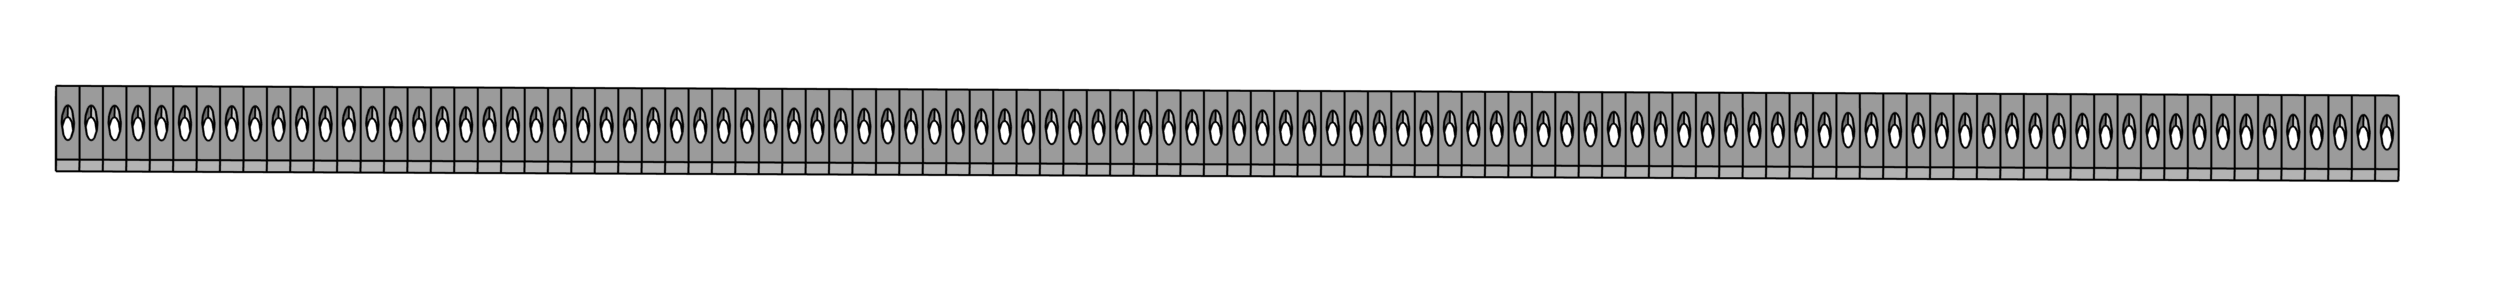
\includegraphics[width=\textwidth]{chapters/results/long_waveguide_geom.png}
	% 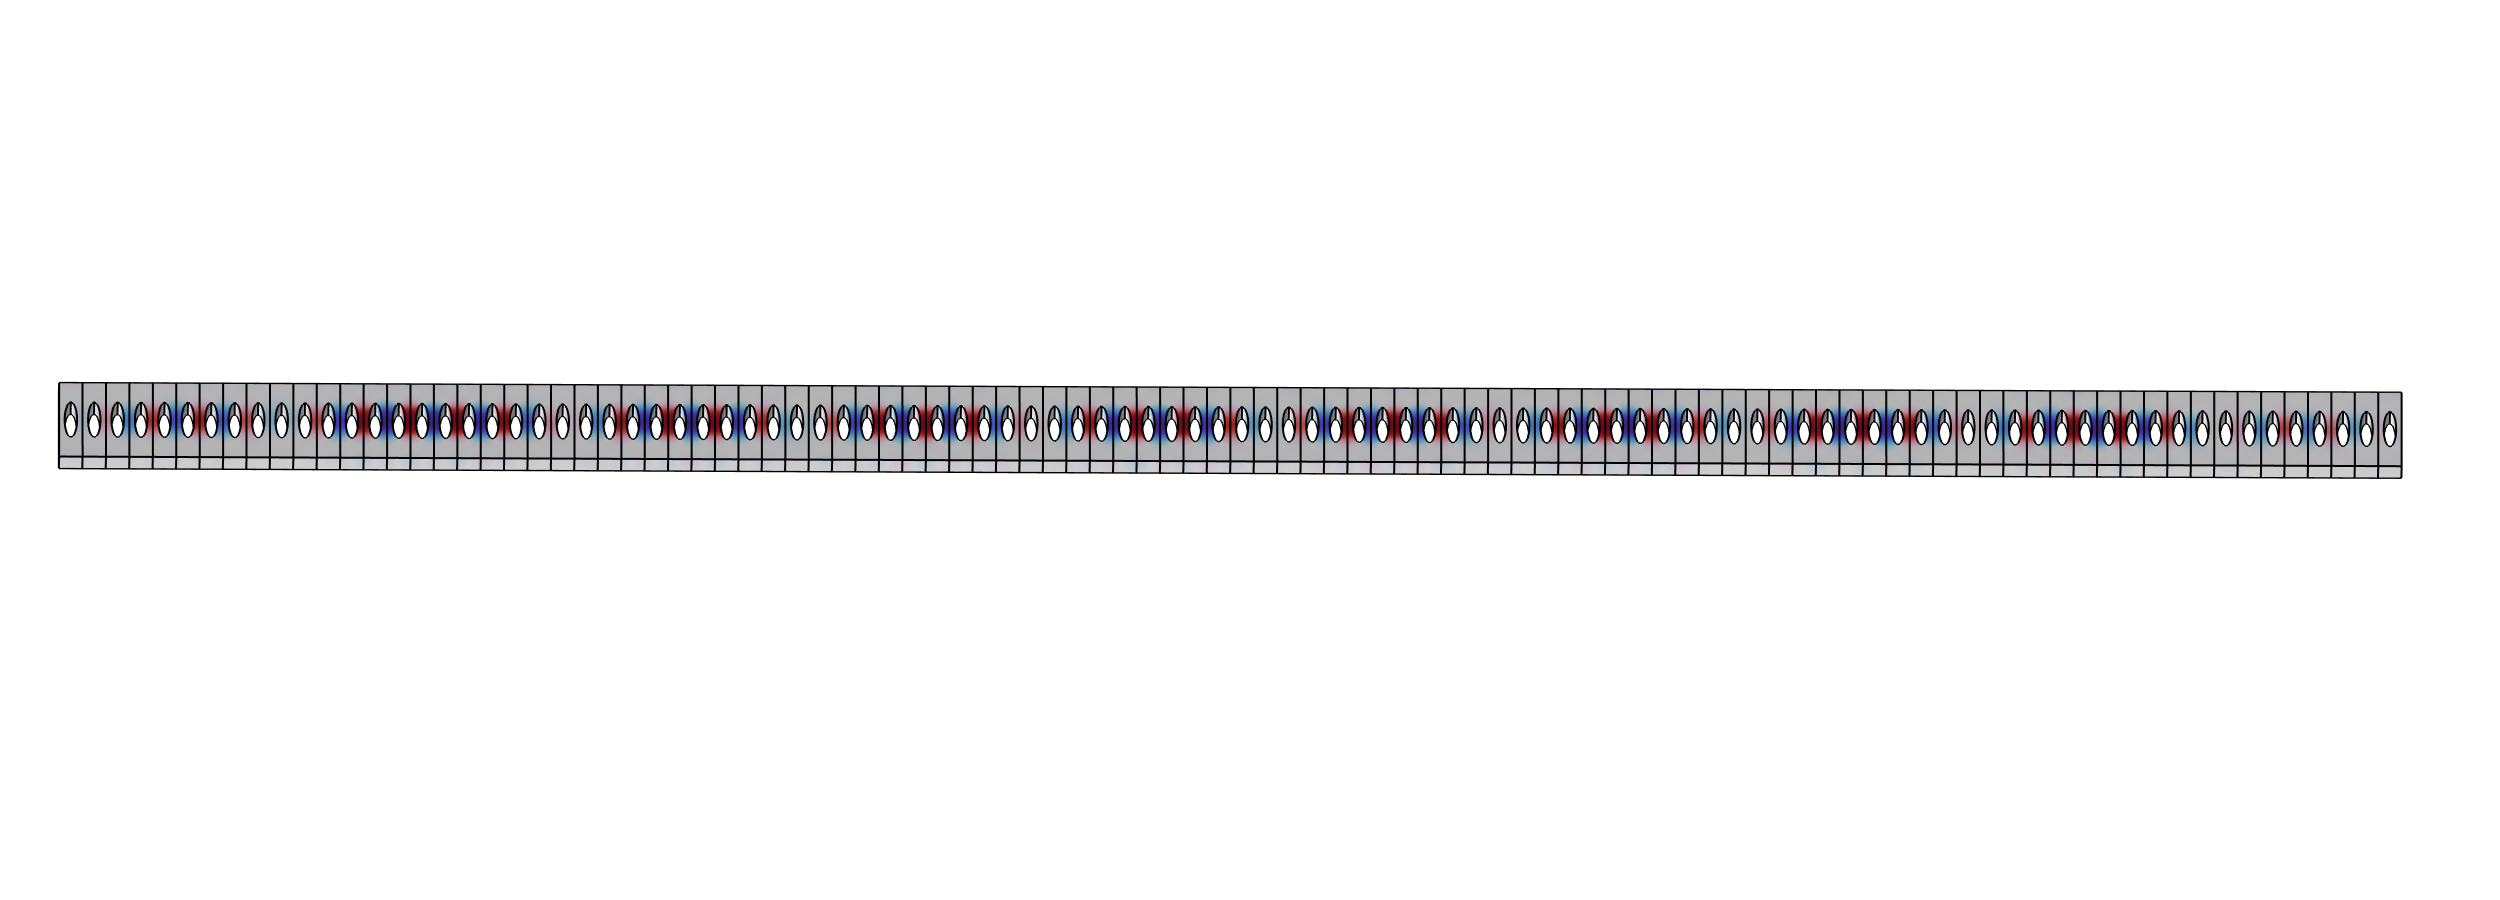
\includegraphics[width=\textwidth]{chapters/results/long_waveguide_v_d=5_s=0.02.png}
	% 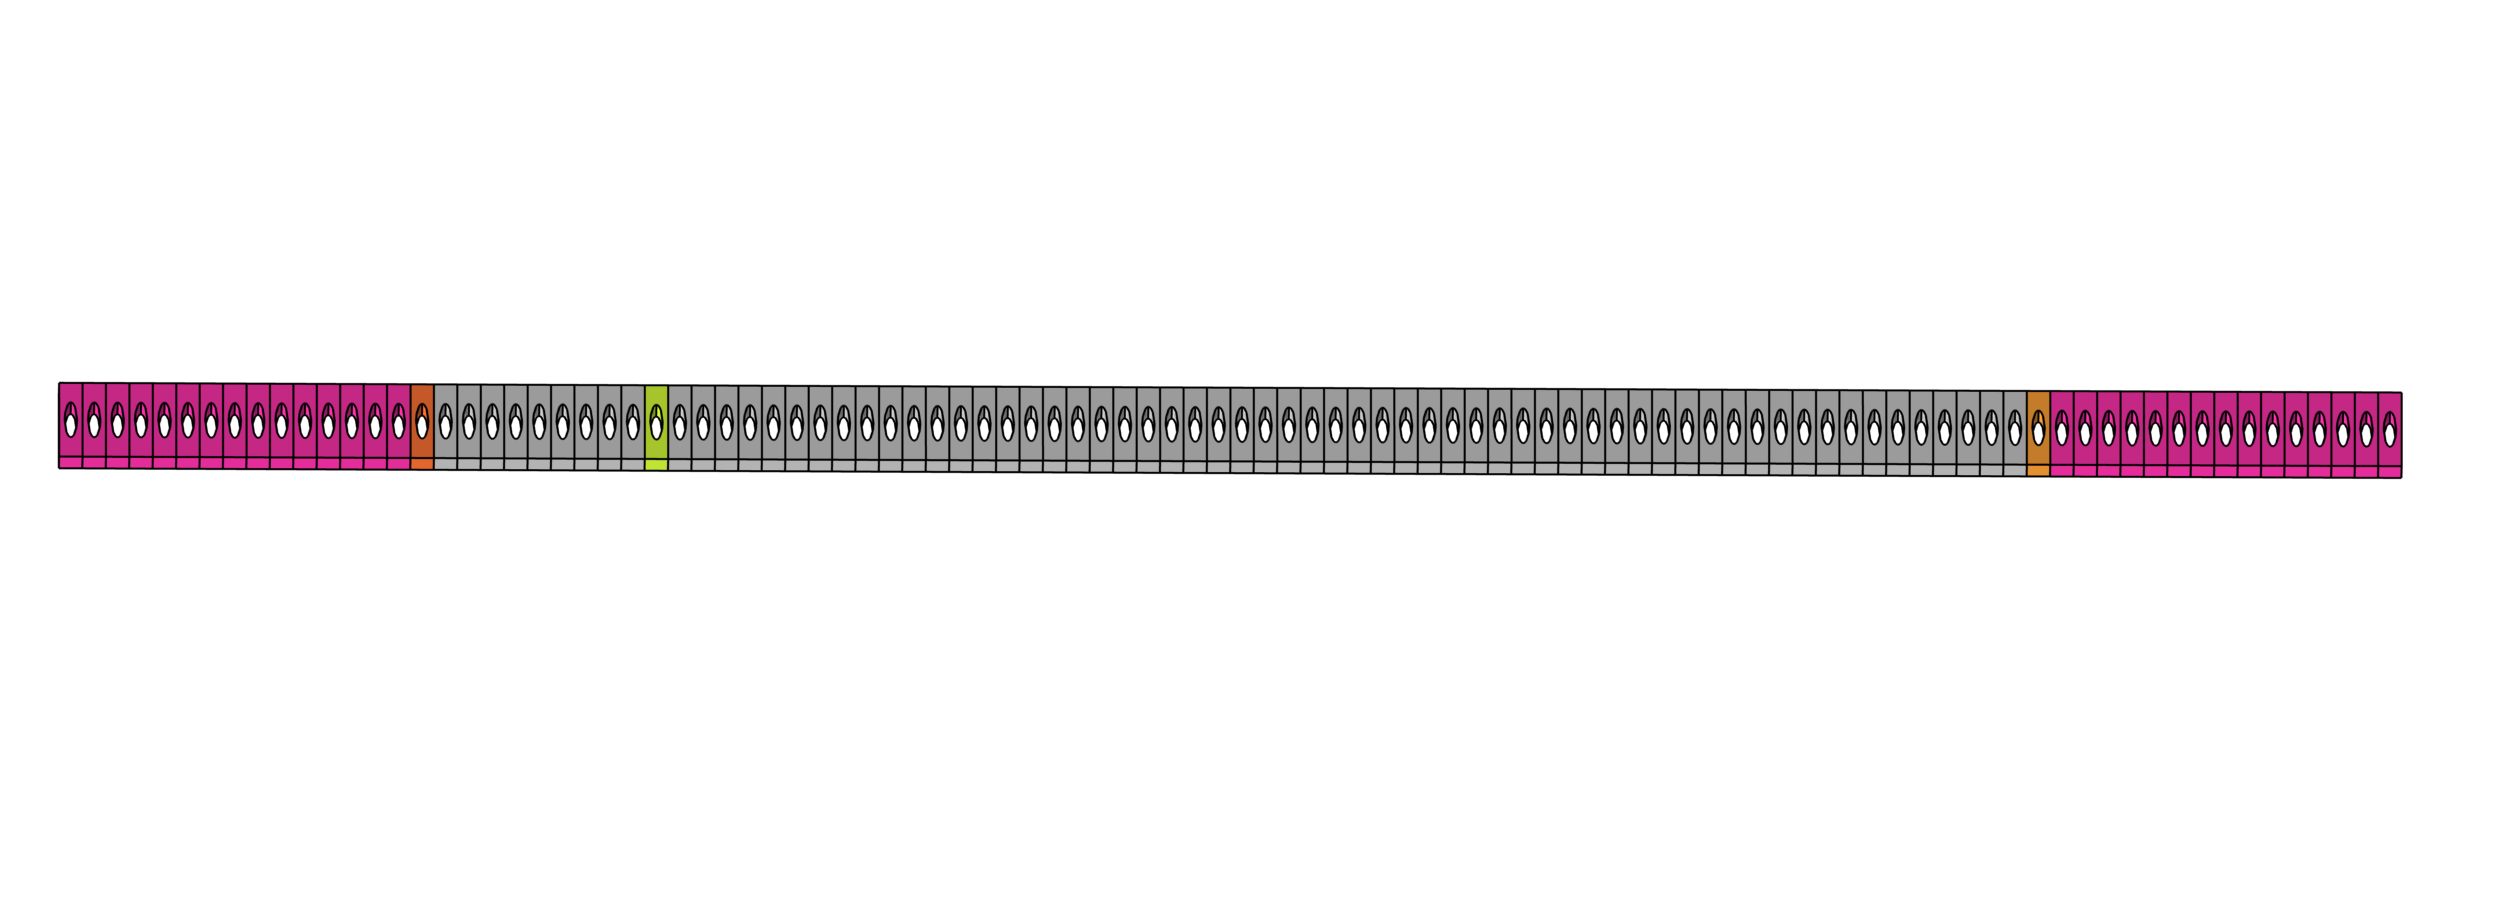
\includegraphics[width=\textwidth]{chapters/results/long_waveguide_selections.png}
	\caption{%
		This figure shows the long waveguide used for the \gls{pml} simulations
		as wells as validating the excitation method.
	}%
	\label{fig:long_waveguide}
\end{figure}

\subsection{Excitation}

The fact that the excitation was almost solely in the desired mode was verified
in two ways.
Firstly, as detailed in \cref{sec:excitation_method}, $a$ and $b$ in $u = a u_m
+ b u_r$ was computed.
The result was that $a = 1.166$ and $b = 0.0327$.
Thus $99.92\%$ of the energy was in the desired mode.
Secondly, a fourier transform of the y-component of the displacement field was
made.
This can be seen in \cref{fig:v_ft}.
The other modes that could be excited at this frequency have very different wave
vectors, which means that they would show up as separate peaks somewhere around
$0.4 \pi / a$ and $0.1 \pi / a$.
Since no other peaks can be seen, this further supports the result that only the
desired mode is excited.

\begin{figure}[htpb]
	\centering
	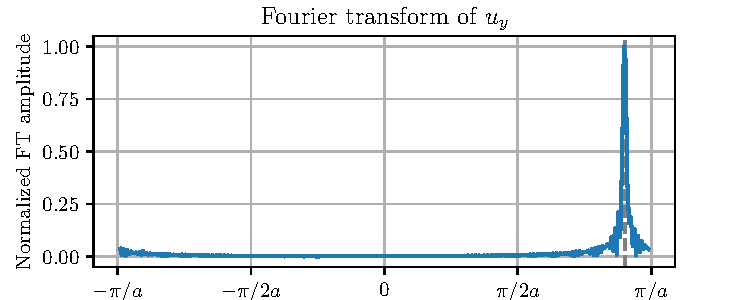
\includegraphics{chapters/results/ft_figure.pdf}
	\caption{%
		Fourier transform of the y-component of the displacement field.
		It clearly shows one wave traveling forward with a k-vector of
		$0.9 \pi / a$, where the dashed gray line is.
		Since the closest other mode at this frequency is at
		$k_y \approx 0.4 \pi / a$, where no peak is visible, it is concluded
		that solely the desired mode is excited.
	}%
	\label{fig:v_ft}
\end{figure}

\subsection{PML investigation}

\Cref{fig:pml_sweep1} shows the amplitude of the reflection,
quantified as the peak height relative to the forward propagating wave,
for different profiles.
These figures fit well with the three types of reflection mentioned previously.
The leftmost plot in \cref{fig:pml_sweep_sd} shows that all of the different
shapes yield reflections when the derivative at the beginning of the \gls{pml}
is around \num{3e-4}, which indicates that the reflections are dominated by
effects from the sudden start of the \gls{pml}.
On the other end, the increase in reflection amplitude come from
waves reaching the end of the \gls{pml} and getting reflected there.
The third type of reflection seems to only be noticeable for $d \leq 4$.
It is also worth noticing that with lower $d$, the plateau where neither of the
first two kinds of reflections are significant is broader.
Since $d=5$ was the lowest $d$ to show no signs of the third type of reflection,
that was chosen for the shape of the \gls{pml} profile.
After that, we investigated how short we could make the it while retaining
low reflections. \Cref{fig:pml_sweep_sn} shows $s$ sweeps for different $n$.
To achieve a short yet functional \gls{pml}, $d=5$, $s=0.03$ and $n=20$ was
chosen.
For $n=15$, reflections from the beginning start to become significant before
the reflections from the end have waned.

\begin{figure}[htpb]
	\centering
	\begin{subfigure}[]{0.99\textwidth}
	\begin{center}
		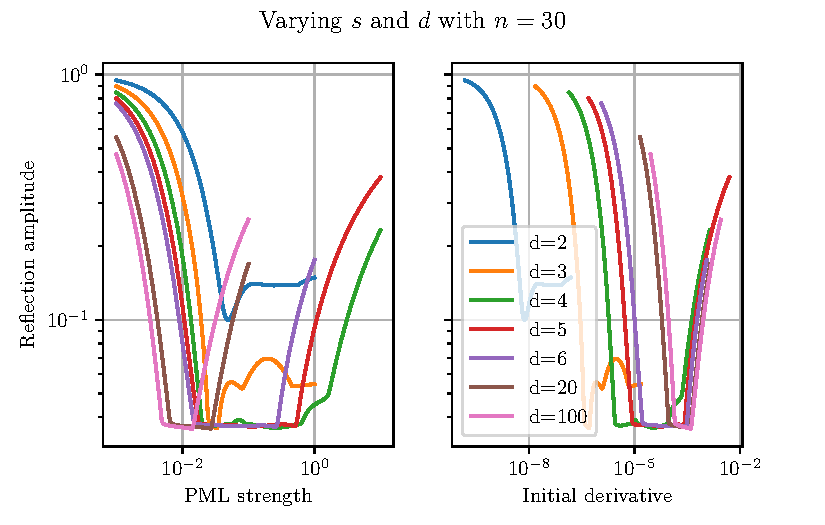
\includegraphics{chapters/results/pml_sweep_sd.pdf}
	\end{center}
	\caption{
		On the left is the reflection amplitude plotted as a function of the
		\gls{pml} strength $s$ for different $d$.
		For $d > 4$ there are two sources of reflection:
		for small $s$ reflection at the end of the \gls{pml} occurs,
		and for large $s$, there is reflection at the beginning.
		The right figure makes it clear that it is the slope at the beginning of
		the \gls{pml} that matters, since the point at which it becomes
		significant is the same for all $d$.
	}
	\label{fig:pml_sweep_sd}
	\end{subfigure}%

	\begin{subfigure}[]{0.99\textwidth}
	\begin{center}
		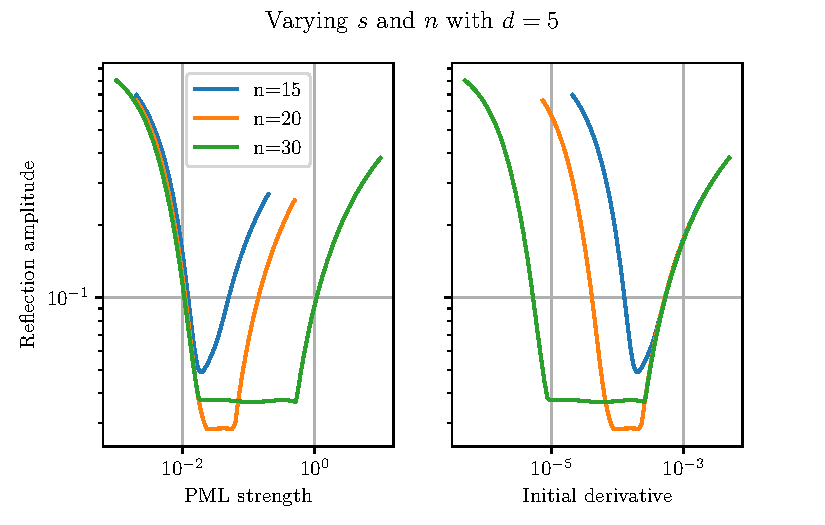
\includegraphics{chapters/results/pml_sweep_sn.pdf}
	\end{center}
	\caption{
		This is the same as \cref{fig:pml_sweep_sd} but with varying $n$.
		For $n=15$, the reflections from the beginning do not subside before the
		reflections from the end become significant, so at least $n=20$ is
		necessary.
	}
	\label{fig:pml_sweep_sn}
	\end{subfigure}
	\caption{}
	\label{fig:pml_sweep1}
\end{figure}

\section{Continuous optimization}\label{sec:res_cont}

There was a lot of problems with the optimization of the continuous design.
Many optimization runs would end up looking like \cref{fig:bad_cont_conv},
reaching a somewhat performant beamsplitter but invariably declining after some
point.
The figure shows the evolution of the transmitted power in one of the
output arms, as well as the reflected power back into the input.
This has been normalized such that 1 is the power in through the input waveguide.
Thus, an optimal beamsplitter would reach 0.5.
If the powers do not add up, it is because energy is flowing out in a different
mode.
I tested a few different theories on why the algorithm might fail to converge.
The first one was that perhaps the simulations were unstable for the case when
$p\approx 0$. To test this I interpolated between $\rho^\text{si}$ and
\qty{1000}{\kg\per\m^3} instead. However, convergence was still not reached.
The second was that maybe the meshing was too coarse to resolve the design
field properly. However, this was not the case as increasing the meshing did not
change the objective function more than a percent or so, so this wasn't the
cause either.
The last thing I thought of was that comsol was using quadratic shape functions
for the fields. This means that on each finite element of the mesh, the fields
are approximated with quadratic polynomials. Thus, if one computes any third
order spatial derivative, it will be 0 everywhere, and the second order
derivatives will not be very accurate.
In \cref{fig:quad_spline_sine} I show how quadratic splines can give a very good
approximation to a function, while still being a terrible approximation to its
second derivative.
Since I used second derivates in computing my gradient, that also wasn't very
reliable.
One way of solving this is to use higher order shape functions, however this
greatly increases the degrees of freedom, making the problem too computationally
expensive, at least with our hardware and geometry.
Another way is to make the mesh much finer, but this is also too computationally
expensive.
\begin{figure}[htpb]
	\centering
	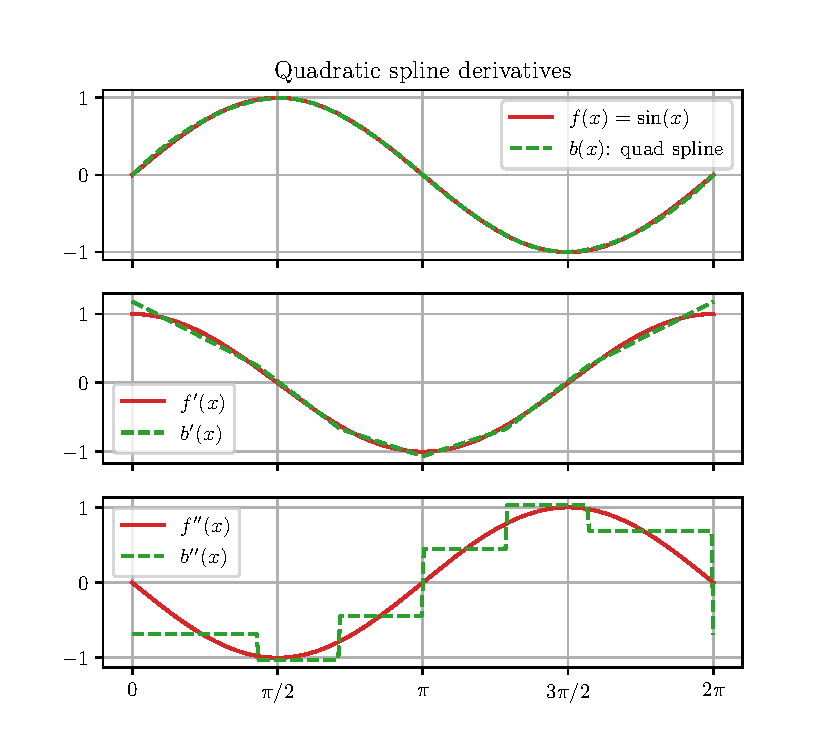
\includegraphics{chapters/results/quad_spline_sine.pdf}
	\caption{%
		This figure shows a quadratic spline approximation to a sine function,
		given eight points on the function. Even though the spline approximates
		the sine function very well, the second derivative approximation is
		terrible.
	}%
	\label{fig:quad_spline_sine}
\end{figure}

However, there was another way:
using the built in COMSOL function \mintinline{c}+fsens+ for computing
the gradient, convergence was obtained.
\Cref{fig:cont_conv1} shows the performance evolution of this optimization run.
At iteration 467, the model was deemed to have converged and as described in
\cref{sec:m_optimization}, a sigmoid function with $r=0.1$ was applied and optimization
continued.
At iteration 615, the model again seemed converged and $r$ was set to $0.05$.
Finally, at iteration 830, near perfect performance was reached and optimization
was terminated.
\Cref{fig:cont_design1} shows the design field after convergence for each of the
three stages.

\begin{figure}[htpb]
	\centering
	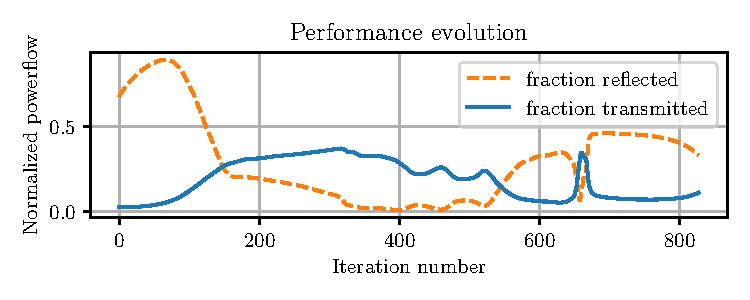
\includegraphics{chapters/results/conv_22.pdf}
	\caption{%
		Non-converging optimization example. The blue curve shows the
		transmitted power in one of the output arms as a function of iteration,
		while the yellow shows the power reflected back out through the input.
		The cases where two times the blue plus the yellow isn't 1.0 is
		explained by power exiting through a different mode.
	}%
	\label{fig:bad_cont_conv}
\end{figure}

\begin{figure}[htpb]
	\centering
	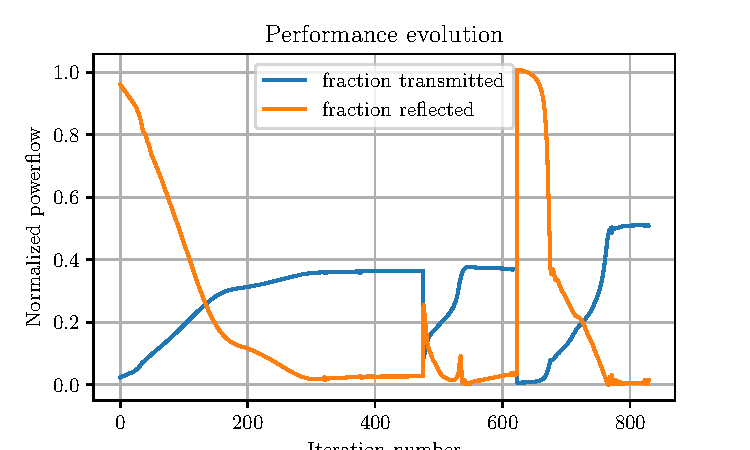
\includegraphics{chapters/results/conv_31.pdf}
	\caption{
		Similar to \cref{fig:bad_cont_conv},
		but at iteration 467 and 615, a sigmoid function was abruptly applied
		to the design field, which causes the dips.
		The final device was a near perfect beamsplitter, with less than 1 \% of
		the power begin reflected, and nothing being scattered into other modes.
	}%
	\label{fig:cont_conv1}
\end{figure}

\begin{figure}[htpb]
	\centering
	\includegraphics{chapters/results/interpolation_fields_468615830.pdf}
	\caption{This figure shows the interpolation field at iteration 467, 615,
		and 830. It is clearly seen that the device becomes closer and closer to
		being binary.
	}%
	\label{fig:cont_design1}
\end{figure}

\section{Level-set optimization}\label{sec:res_bin}

% Because the continuous optimization didn't converge until rather late,
% I did not have time to explore the level-set optimization as much as I would
% have liked.
The initial contour of the device was taken as the 0.5-isocontour of the final
design field from the continuous optimization.
\Cref{fig:bin_conv} shows the convergence plot for the level-set optimization,
and \cref{fig:bin_design} shows the final device.
Something to note is that the device does seem to be rather sensitive;
a shift of only a nanometre can greatly change the device performance.
Therefore the $\alpha$ chosen for the algorithm had to be set as low as
\qty{0.5}{\nm}.

\begin{figure}[htpb]
	\centering
	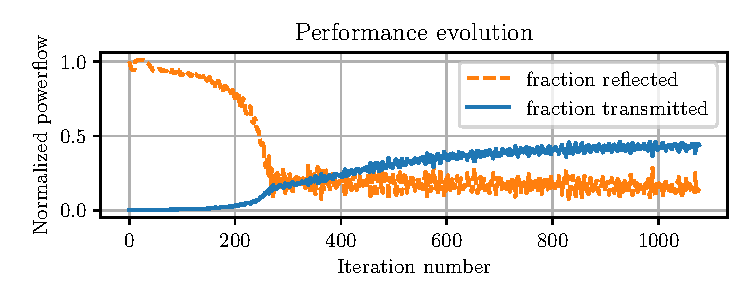
\includegraphics{chapters/results/conv_tmp.pdf}
	\caption{Still running simulation :D}%
	\label{fig:bin_conv}
\end{figure}

\begin{figure}[htpb]
	\centering
	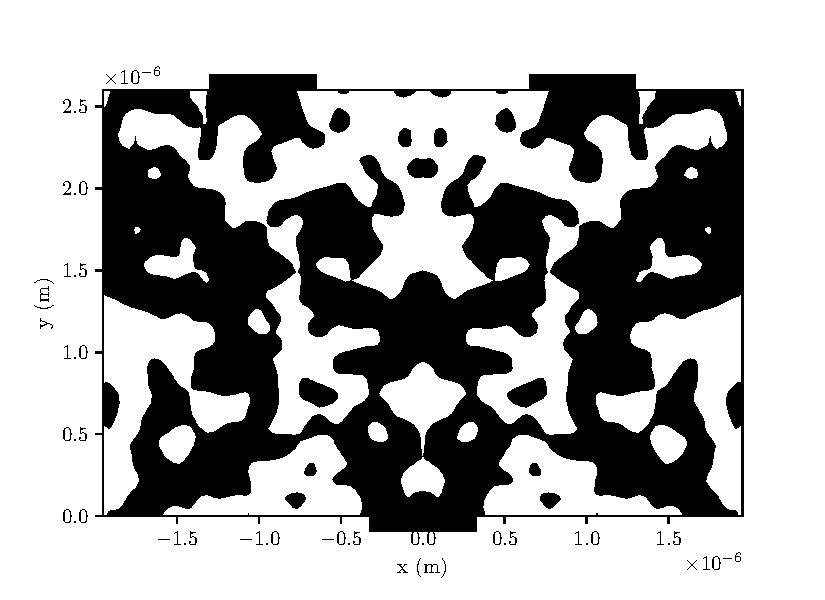
\includegraphics{chapters/results/bin_design_tmp_254.pdf}
	\caption{%
		The current best design from the level-set simulations (but they are
		still running:)
	}%
	\label{fig:bin_design}
\end{figure}

\chapter{Concluding Remarks}

Phononics has the potential to become a vital part of both quantum and
classical information processing architecture, but devices are still limited to
those that can be investigated through analytical means and/or be optimized with
brute force methods. This study set out to investigate whether inverse design
with adjoint simulation could be used to design so far unrealized devices and
enable little explored applications.

We first examined theoretically the applicability of adjoint simulation on
phononics, from which we concluded that the methods should work.
The second aim of this thesis was to demonstrate the utility of this method by
designing a phononic beamsplitter as a proof-of-concept.
To do that, the process was split into two stages, a first where the material
was allowed to vary continuously, to obtain an approximate design as the
starting point for the second stage, where a binary design was
enforced using level-set methods.
The continuous optimization yielded near perfect performance, validating the
theoretical derivations.
The level-set optimization never did achieve perfect performance, but
good performance was still reached.
These results indicate that the inverse design concept can be useful for
designing traveling-wave phononic devices going forward.
We remain hopeful that the problems with the latter stage can be solved
though, which would be a major step forward.

\section{Future Research}

There are a great number of potential paths that can be explored from this
point, and the positive results presented here warrant further efforts in this
area.
One important improvement that should be investigated is the sensitivity of the
device to small changes in the design.
If it is very sensitive, imperfections in fabrication could be detrimental to
the devices performance.
There may be some ways of mitigating this however, for example by running
multiple simulations with small perturbations in the design and averaging them
to obtain the objective function.
Another potential path of exploration is the limiting of the feature size.
This could be done by augmenting the objective function, adding
a pure part that punishes small features.

After these issues have been solved, one could make the model more realistic,
for example by adding a substrate instead of the fixed bottom used in this
thesis.
Ultimately, the designs need to be fabricated and measured experimentally as
well to confirm that the designed devices are functional.

In addition to method improvements, another path is to apply this to designing
other types of devices. For example, waveguide bends seem to be well suited for
this type of design, and would be useful if one wishes to use phononic
waveguides for routing excitations around on a chip. It may also be possible to
inverse design hybrid devices that use both optics and mechanics for example,
though that would likely require a significant effort.


% REFERENCES / BIBLIOGRAPHY
% Use a separate file to be able to exclude with \includeonly
\printbibliography[title={\thesisBibName}, heading=bibintoc]


% APPENDICES
\cleardoublepage
\appendix
\pagenumbering{bychapter}
% CREATED BY MAGNUS GUSTAVER, 2020
\chapter{First appendix}
\lipsum[1]

\chapter{Second appendix}
\lipsum[1]


% LAST PAGE
\if\thesisStatus f
    % LAST PAGE
\begingroup % make parskip changes etc. local

\cleardoublepage
\pagenumbering{gobble}
\thispagestyle{empty}

\if\thesisLayout 2 % extra blank page in two-sided layout
    \leavevmode\newpage
    \thispagestyle{empty}
\fi

% Header Last Page
\vtop{
    \null\vspace{-27.5mm}
    \centerline{\textcolor{thesisHeaderColor}{\rule{1.28\textwidth}{28mm}}}
    \null\vspace{-9mm}
    \centerline{\textcolor{headerBrown}{\rule{1.28\textwidth}{4pt}}}
    \vspace{187mm}
    \if\thesisType M
    \centerline{
\includegraphics[width=0.2\pdfpagewidth]{template/figures/AvancezChalmersU_black_centered.eps}}
    \fi
    \if\thesisType B
    \centerline{
\includegraphics[width=0.2\pdfpagewidth]{template/figures/AvancezChalmers_black_centered.eps}}
    \fi
    \vspace{-220mm}
}

%\addtolength{\voffset}{2cm}
\renewcommand{\familydefault}{\sfdefault} \normalfont % Set cover page font
\vspace*{-4.5cm}
\noindent
\textcolor{white}{\footnotesize \textbf{\MakeUppercase{\thesisDepartment}}\\
\textbf{\MakeUppercase{\thesisUniversity}} \\
\thesisLocation \\
\href{\thesisUniversityURL}{\textcolor{white}{\thesisUniversityURL}}}

\endgroup

\fi

\end{document}
